%----------------------------------------------------------------------------------------
%	PACKAGES AND OTHER DOCUMENT CONFIGURATIONS
%----------------------------------------------------------------------------------------

	\documentclass[a4paper, 11pt, oneside]{book}

	\usepackage[sc]{mathpazo} % Use the Palatino font
	\usepackage[utf8]{inputenc}
	\usepackage[spanish, es-tabla]{babel}
	\decimalpoint
	
	\usepackage{lipsum}
	\usepackage{graphicx}
	\usepackage[T1]{fontenc} % Use 8-bit encoding that has 256 glyphs
	\linespread{1.15} % Line spacing - Palatino needs more space between lines
	%\usepackage{microtype} % Slightly tweak font spacing for aesthetics
	%
	\usepackage[hmarginratio=1:1,left=20mm, top=22mm]{geometry} % Document margins
	%\usepackage{multicol} % Used for the two-column layout of the document
	\usepackage[hang, small,labelfont=bf,up,textfont=it,up]{caption} % Custom captions under/above floats in tables or figures
	\usepackage{mathtools}
	%\usepackage{booktabs} % Horizontal rules in tables
	\usepackage{float} % Required for tables and figures in the multi-column environment - they need to be placed in specific locations with the [H] (e.g. \begin{table}[H])
	\usepackage{hyperref} % For hyperlinks in the PDF
	\usepackage{appendix}
	\usepackage{subcaption}
	%\usepackage{wrapfig}
	%%\usepackage[]{mcode} % For embebing matlab code
	%\usepackage[makeroom]{cancel}
	%
	%%\usepackage{lettrine} % The lettrine is the first enlarged letter at the beginning of the text
	%\usepackage{paralist} % Used for the compactitem environment which makes bullet points with less space between them
	%
	%\usepackage{abstract} % Allows abstract customization
	%\renewcommand{\abstractnamefont}{\normalfont\bfseries} % Set the "Abstract" text to bold
	%\renewcommand{\abstracttextfont}{\normalfont\small\itshape} % Set the abstract itself to small italic text
	%%%
	%\usepackage{titlesec} % Allows customization of titles
	%%\renewcommand\thesection{\Roman{section}} % Roman numerals for the sections
	%%\renewcommand\thesubsection{\Roman{subsection}} % Roman numerals for subsections
	%\titleformat{\section}[block]{\large\scshape\centering}{\thesection.}{1em}{} % Change the look of the section titles
	%\titleformat{\subsection}[block]{\large\centering}{\thesubsection.}{1em}{} % Change the look of the section titles
	%
	%\usepackage{fancyhdr} % Headers and footers
	%\pagestyle{fancy} % All pages have headers and footers
	%\fancyhead{} % Blank out the default header
	%\fancyfoot{} % Blank out the default footer
	%\fancyhead[C]{Titulo Corto% based on TRACS 
	%\hspace{4pt} $\bullet$ \hspace{4pt} MES ANO } % Custom header text
	%\fancyfoot[RO,LE]{\thepage} % Custom footer text
	%
	\usepackage{cite}
	\usepackage{listings}
	\usepackage{color}

	\graphicspath{{../Graphics/}}
	%
	%\DeclareGraphicsExtensions{.pdf,.png,.jpg} % Graphics type

	\newcommand{\gs}{encendido por ganancia}
	\newcommand{\ibias}{I_{bias}}
	\newcommand{\chirp}{$\nu_{chirp}$}
	\newcommand{\I}{corriente de inyecci\'on $I(t)$}
	\newcommand{\n}{$N(t)$}
	\newcommand{\s}{$S(t)$}
	\newcommand{\fase}{fase \'optica $\Phi(t)$}
%----------------------------------------------------------------------------------------
%	   METADATA
%----------------------------------------------------------------------------------------

	%\title{
	%	\selectfont\textbf{TITULO}% Article title
	%}

	%\author{
	%	\textsc{Jaime Diez Gonzalez-Pardo}\\
	%	%\thanks{A thank you or further information}\\ % Your name
	%	\fontsize{28pt}{10pt} Universidad de Cantabria \\ % Your institution
	%	%\thanks{A thank you or further information}\\[2mm] % Your name
	%	\normalsize gsdfgdfgdfgatura \\ 
	%	\normalsize{Compañeros:} \textsc{NOMBRE COMPANEROS }\\
	%	%\vspace{5mm}
	%}

	%\date{\today}
%----------------------------------------------------------------------------------------
%      · DOCUMENT
%----------------------------------------------------------------------------------------

	\begin{document}

		\begin{titlepage} 

			\newcommand{\HRule}{\rule{\linewidth}{0.5mm}} 
			
			\center % Centre everything on the page
			
			%------------------------------------------------
			%	Headings
			%------------------------------------------------
			
				%------------------------------------------------
				%	Logo
				%------------------------------------------------
				
					\begin{figure}[H]
						\centering
						
\includegraphics[scale=0.6]{download.png}
					\end{figure}

					\textsc{\LARGE Facultad de Ciencias}\\[1.5cm] 
			
			
			%------------------------------------------------
			%	Title
			%------------------------------------------------
			
				\HRule\\[0.4cm]
				
				{\huge\bfseries Simulación de peines de frecuencia óptica generados por láseres de semiconductor}\\[0.8cm] % Title of your document

				{\huge Simulation of optical frequency comb generated by semiconductor lasers}\\[0.4cm] % Title of your document
				
				\HRule\\[1.5cm]

				{\Large Trabajo de Fin de Grado para acceder al}\\[0.4cm]

				{\LARGE\bfseries Grado en Física}\\[3cm]
			
			%------------------------------------------------
			%	Author(s)
			%------------------------------------------------
			
				\begin{flushright}
					\large
					\textit{Autor}\\
					Jaime \textsc{DÍEZ GONZÁLEZ-PARDO} \\ % Your name
					\large
					\textit{Director}\\
					Dr. Ángel \textsc{VALLE GUTIERREZ} % Supervisor's name
				\end{flushright}
			
			%------------------------------------------------
			%	Date
			%------------------------------------------------
			
				\vfill\vfill\vfill % Position the date 3/4 down the remaining page
				
				{\large\today} % Date, change the \today to a set date if you want to be precise
				
			%----------------------------------------------------------------------------------------
			
				\vfill % Push the date up 1/4 of the remaining page
		
		\end{titlepage}

			\begin{center}
				\textbf{ \large Agradecimientos}
			\end{center}
					
				Quiero dar las gracias a mi director de trabajo, el Prof. \'Angel Valle, no solo por toda la dedicaci\'on y apoyo mostrados en todo momento y por introducirme en el desconcocido mundo de la din\'amica no lineal, sino tambi\'en por animarme durante los \'ultimos d\'ias a realizar el \'ultimo gran esfuerzo, arrastr\'andole a \'el en ello.  \\
					
				Tambi\'en quiero dar las gracias a todas las personas que me han introducido en la f\'isica. En especial a mi profesor de m\'atematicas de secundaria, Feliz Horga, por aprovechar cualquier ocasi\'on para salirse del temario y enseñarnos las cosas tan bonitas que esconde la física, y a mi hermano Álvaro por transmitirme con tanta pasión todo lo que aprendia de física. \\

				Agradecerle a mi hermana, y en especial a mi padre, toda la paciencia que han demostrado tener estándo siempre ahi. Gracias tambiçén a toda la gente que me ha acompañado durante estos cuatro años, en especial a Inés que tantas horas me ha aguantado. \\

				Todo lo hago por tí, gracias Mamá.

			\newpage
			\begin{center}
				\textbf{\centering Resumen}
			\end{center}

				En este trabajo se han estudiado las caracteristicas de los peines de frecuencia \'optica en l\'aseres de semiconductor generados mediante las t\'ecnicas de \gs\ e inyecci\'on \'optica. Para ello se ha desarrollado un programa que ha permitido resolver las ecuaciones de balance mediante la implementaci\'on de un modelo num\'erico. Dichas ecuaciones de balance presentan t\'erminos de ruido estoc\'astico por lo que ha sido necesario utilizar m\'etodos de integraci\'on de ecuaciones diferenciales estoc\'asticas para su resoluci\'on.

				En la primera parte del trabajo se ha realizado el estudio de la simulación del l\'aser de semiconductor en solitario, analizando los resultados para el l\'aser en corriente cont\'inua y con \gs. Para el caso del l\'aser \gs\ se ha procedido a caracterizar los peines de frecuencia \'optica en funci\'on de la amplitud $V_{RF}$ y la frecuencia $f_R$ de la corriente inyectada. Se ha observado la creaci\'on y destrucci\'on de los peines a medida que se aumentaba la amplitud, as\'i como una mayor irregularidad para bajas frecuencias.

				En las siguientes partes se ha analizado la generaci\'on de peines de frecuencia \'optica mediante inyecci\'on de luz de un segundo l\'aser, caracterizada por la potencia inyectada $P_{Iny}$ y la diferencia de frecuencias entre ambos l\'aseres $\delta\nu$. Primero se ha estudiado el caso de inyecci\'on \'optica sin \gs, pasando a continuaci\'on a estudiar el caso de combinar ambos m\'etodos. El modelo ha permitido determinar las diferentes regiones dinámicas para distintas inyecciones, pudiendo identificar regiones con bifurcaciones de Hopf y de doblamiento de periodo.

				Se ha obtenido un excelente acuerdo entre los resultados de la simulación y los experimentales \cite{Chaves19}, mostrando la gran capacidad predictiva del modelo.
		
			\begin{center}
				\textbf{Palabras clave:} L\'aser de Semiconductor, Ecuaciones de Balance, Encendido por Ganancia, Inyecci\'on \'Optica, Peines de Frecuencia \'Optica.
			\end{center}

		\newpage
			\begin{center}
				\textbf{Abstract}
			\end{center}

				In this dissertation we have studied the characteristics of the optical frequency combs in semiconductor lasers generated by gain-switching and optical injection. A program has been developed to solve rate equations by implementing a numerical model. These rate equations present terms of stochastic noise, being necessary to use methods of integration of stochastic differential equations for their resolution. 
				
				In the first part of the work, the study of the simulation of the semiconductor laser alone has been carried out, analyzing the results for the laser in continuous wave and with gain-switching. In the case of the laser in gain-switching, the optical frequency combs have been characterized according to the amplitude $V_{RF}$ and the frequency $f_R$ of the injected current. The creation and destruction of combs has been observed as the amplitude was increased, as well as a greater irregularity for low frequencies.

				In the following parts the generation of optical frequency combs has been analyzed by means of optical injection from a second laser, characterized by the injected power $P_{Iny}$ and the detuning between both lasers' frequency $\delta\nu$. First, the case of optical injection without gain-switching has been studied, going on to study the combination of both methods. The model has allowed to determine the different dynamic regions for different injections, being able to identify regions with period doubling and Hopf bifurcations.

				An excellent agreement has been obtained between the simulation results and the experimental ones \cite{Chaves19}, showing the great predictive capacity of the model.

			\begin{center}
				\textbf{Key words:} Semiconductor Laser, Rate Equations, Gain Switching, Optical Injection, Optical Frequency Combs. 
			\end{center}

		%\thispagestyle{fancy} % All pages have headers and footers

		\tableofcontents

		%\listoffigures

		%----------------------------------------------------------------------------------------
		%	  ARTICLE CONTENTS
		%----------------------------------------------------------------------------------------

			\addtocontents{toc}{\vspace{0.01cm}}
			\chapter{Introducción} % Scope of the project = rad effects + minimization
				\label{Intr}

				El uso de dispositivos el\'ectricos de semiconductor supuso un avance enorme en la tecnolog\'ia, permitiendo desarrollar dispositivos m\'as eficientes y pequeños, conviertiendose en una parte fundamental de nuestra sociedad. Uno de estos dispositivos que han supuesto un gran avance son los l\'aseres de semiconductor, que ha descubierto un enorme campo de estudio, debido a sus importantes propiedades y a la multitud de aplicaciones en diferentes \'areas.

Este trabajo se centra en la creaci\'on de peines de frecuencia \'optica (OFC de sus siglas en ingl\'es) en un l\'aser de semiconductor de emisi\'on lateeral y modo discreto. Estos OFC presentan caracter\'isticas diversas en funci\'on de los par\'ametros que defienen su proceso de creaci\'on, debido a la din\'amica no lineal del sistema del l\'aser.

El objetivo de este trabajo es el estudio computacional del comportamiento de la diferentes regiones din\'amicas de los peines de frecuencia \'optica en l\'aseres de semiconductor con \gs\ e inyecci\'on \'optica. Este estudio permitir\'a entender los procesis f\'isicos relevantes en la formaci\'on de los OFC.

En este cap\'itulo se han introducido los conceptos te\'oricos relevantes de los temas tratados en este trabajo. Se ha realizado una breve introducci\'on sobre los l\'aseres de semiconductor, los procesos estoc\'asticos y la din\'amica no lineal, pasando a continuaci\'on a describir los peines de frecuencia \'optica y dos de los m\'etodos utilizados para su obtenci\'on: el \gs\ y la inyecci\'on \'optica.

	\addtocontents{toc}{\vspace{0.01cm}}
	\section{Láseres de Semiconductor}
		\label{Intr:LsrSmcdtr}
		
		\graphicspath{{./Introduccion/Figures/}}

La caracter\'istica principal de los semiconductores es la separaci\'on o gap entre la banda de valencia y la banda de conducci\'on, con un valor pequeño ($\varepsilon_g  = \varepsilon_C - \varepsilon_V \sim 0.1 - 3$ eV). Al tener un gap pequeño pueden darse saltos entre electrones de la banda de valencia y la banda de conducci\'on, apartir de la mediaci\'on de un fot\'on. Estas interacciones solo se pueden dar para energias del fot\'on $h\nu > \varepsilon_g$.

Las tres posibles formas de interacci\'on luz-materia son la emisi\'on espont\'anea, la emisi\'on estimulada y la absorci\'on. En un material semiconductor a $T = 0$K se tiene la banda de valencia completamente llena y la banda de conducci\'on vac\'ia. Al aumentar la temperatura se pueden dar saltos de los electrones a la banda de conducci\'on debido al pequeño gap. Al situarse un electr\'on en un nivel superior de energ\'ia, \'este tender\'a a volver a su estado de m\'inima energ\'ia recombinandose de nuevo en la banda de valencia, pudiendo emitir un fot\'on en el proceso. Este proceso es el denominado emisi\'on espont\'anea y es muy d\'ebil debido a que cada fot\'on puede tener diferente fase y direcci\'on.

	\begin{figure}[H]
		\centering
		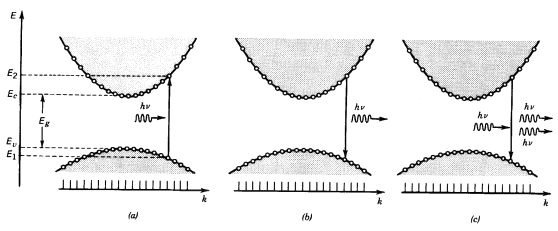
\includegraphics[width=0.6\linewidth]{BV-BC.png}
		\caption{\label{Img:Saleh-BV-BC}Esquema de bandas con las tres interacciones luz-materia en un semiconductor: (a) absorci\'on, (b) emisi\'on espont\'anea y (c) emisi\'on estimulada \cite{saleh2019fundamentals}.}
	\end{figure}

Debido a la poca intensidad de la emisi\'on espont\'anea, el proceso clave para los l\'aseres de semiconductor, al igual que para el resto, es el dominio de la emisi\'on estimulada. Si sobre el material con un electr\'on excitado en la banda de conducci\'on, se incide con un fot\'on de frecuencia $\nu_0$ igual a la diferencia de energ\'ias entre el estado excitado del electr\'on y el fundamental, se forzar\'a al electr\'on a decaer al nivel de menor energ\'ia. El fot\'on emitido en la recombinaci\'on del electr\'on tendr\'a las mismas propiedades que el fot\'on incidente, puediendo estos dos fotones interactuar con m\'as electrones excitados y as\'i producir la amplificaci\'on de la radiaci\'on incidente. Sin embargo, para que esta amplificaci\'on continue, debe haber una cantidad suficiente de electrones excitados. Para ello se utilizan fuentes de bombeo para obtener la inversi\'on de poblaci\'on.

El medio en el cu\'al se producen la mayor parte de emisiones espont\'aneas se denomina medio activo y para los l\'aseres de semiconductor suelen ser heteroestructuras por capas conuna uni\'on $pn$ en la direcci\'on de avance de la corriente. Cuando la corriente inyectada al l\'aser es suficientemente grande, se obtienen suficientes electrones en la banda de conducci\'on para amplificar la luz. Una ventaja de los l\'aseres de semiconductor es su alta densidad de electrones, que permiten alcanzar grandes valores para la ganancia y unas distancias pequeñas de la cavidad, del orden de $\sim 1$ mm.

La direcci\'on del medio activo con respecto al haz de luz emitido permite diferenciar entre dos tipos de l\'aseres de semiconductor. Los l\'aseres de emisi\'on vertical (VCSEL) presentan el medio activo ortogonal al haz de luz mientras que para los de emisión lateral el medio activo es paralelo al haz de luz emitida. 

NO SE SI HE DE MENCIONAR ALGO SOBRE LASERES DE MODO DISCRETO


	\addtocontents{toc}{\vspace{0.01cm}}
	\section{Procesos Estocásticos}
		\label{Intr:PrcsEstcs}
		
		
	%En esta seccion se va a hablar de los procesos estocasticos del problema y de las ecuaciones diferenciales estocasticas, asi como de su resolucion.
	

Los procesos estoc\'asticos permiten describir la evoluci\'on temporal de un sistema con comportamiento aleatorio a partir de la probabilidad estad\'istica de \'este \cite{gardiner1985handbook}. El ejemplo m\'as relevante de los procesos estoc\'asticos es el movimiento Browniano, que describe la evoluci\'on de la posici\'on de una part\'icula en el seno de un fluido, con impactos frecuentes e irregulares (aleatorios) con las part\'iculas del fluido. El movimiento Browniano viene definido por la ecuaci\'on de Langevin y as\'i, se puede describir su evoluci\'on realizando el promedio con diferentes perturbaciones aleatorias. Para el caso de un experimento esto equivaldr\'ia a realizar el promedio de los resultados, repitiendo el experimento un n\'umero suficiente de veces, hasta obtener la distribuci\'on de probabilidad del proceso.  Una forma alternativa de resoluci\'on del movimiento Browniano es a partir de la ecuaci\'on de Fokker-Planck. Para la evolución unidimensional esta ecuación es la ecuacion de difusión \ref{eq:Fokker-Plank} que da la probabilidad de que la posición de la partícula, $\overline{\underline{X}}(t)$, esté en $x$ en un tiempo $t$ con $P = P(x, t)$, donde $D$ es el coeficiente de difusión.

	\begin{equation}
		\frac{\partial P}{\partial t} = D \frac{\partial^2 P}{\partial x^2}
		\label{eq:Fokker-Plank}
	\end{equation}

	Otro ejemplo de proceso estoc\'astico es el de luz emitida por un l\'aser, cuya principal fuente de aleatoriedad viene dada por la emisión espontánea. Cuando la distribuci\'on de probabilidad del sistema para un conjunto de variables, no varia para un desplazamiento en el tiempo, se dice que se trata de un proceso estoc\'astico estacionario y se cumple que:
	
	\begin{equation}
		\begin{matrix}
			P(x_1, t_1,..., x_n, t_n) = P(x_1, t_1+\delta t,..., x_n, t_n+\delta t) \\ \\
			P(x_1, t_1, x_2, t_2) = P(x_1, x_2, \tau) \rightarrow \textrm{      con    } \tau = t_2 - t_1
		\end{matrix}
	\end{equation}



As\'i, la autocorrelaci\'on $R(t_1, t_2) = E\left[\overline{\underline{X}}(t_1)\overline{\underline{X}}(t_2)\right] = R_\tau$ depende solo de la diferencia de tiempos $\tau = t_1 - t_2$. En la ecuación anterior $E\left[\overline{\underline{X}}(t_1)\overline{\underline{X}}(t_2)\right]$ es el valor medio del producto de $\overline{\underline{X}}(t_1)$ por $\overline{\underline{X}}(t_2)$ sobre distintos resultados del experimento. Para un proceso estacionario, para el que la media es contante respecto a $t$, se puede relacionar la autocorrelaci\'on y el espectro de potencia $S(\omega)$ mediante el teorema de Kintchine, y la transformada de Fourier.

	\begin{equation}
		\begin{matrix}
			S(\omega) = \int_{-\infty }^{\infty } R(\tau) e^{-i\omega\tau} \mathrm{d} \tau \\ \\
			S(\omega) = \lim_{T \rightarrow 0} E\left[\frac{1}{2T} \left| \int_{-T }^{T} \overline{\underline{X}}(t) e^{-i\omega t} \mathrm{d} t \right| ^2 \right ]
		\end{matrix}
		\label{eq:kintchine}
	\end{equation}

%En los procesos estoc\'asticos Markovianos las probabilidades condicionadas est\'an determinadas por el conocimiento del pasado m\'as reciente , pues $\tau_1 \geq \tau_2 \geq \textrm{...} \geq \tau_n$. Para que un proceso estoc\'astico sea Markoviano ha de cumplir las condiciones de \ref{eq:Markiviano}, pudiendo obtener la ecuaci\'on de Chapman Kolmog\'orov \ref{eq:Ch-Kgr}.

	%\begin{equation}
	%	\begin{matrix}
	%		P(x_1, t_1, x_2, t_2, ...| y_1, \tau_1, y_2, \tau_2, ...) = P(x_1, t_1, x_2, t_2, ...| y_1, \tau_1) \\ \\
	%		P(x_1, t_1, x_2, t_2, ..., x_n, t_n) = P(x_1, t_1|x_2, t_2)P(x_2, t_2|x_3, t_3)...P(x_n-1, t_n-1|x_n, t_n)P(x_n, t_n)
	%	\end{matrix}
	%	\label{eq:Markiviano}	
	%\end{equation}

	%\begin{equation}
	%	P(x_1, t_1|x_3, t_3) = \int \mathrm{d}x_2 P(x_1, t_1|x_2, t_2)P(x_2, t_2|x_3, t_3)
	%	\label{eq:Ch-Kgr}
	%\end{equation}

Hay un tipo especial de procesos estocásticos en los que las probabilidades condicionadas están determinadas por el conocimiento del pasado más reciente, los procesos Markovianos. Para ellos la densidad de probabilidad de que el proceso tome el valor $z$ en $t$, sabiendo que tomó el valor $y$ en $t'$ ($P(z, t| y, t')$), satisface la ecuaci\'on de Fokker Plank \ref{eq:FPE}.

	\begin{equation}
		\frac{\partial P(z, t|y, t'))}{\partial t} = \frac{\partial }{\partial z}\left(A(z, t)P(z, t|y, t') \right ) + \frac{1}{2} \frac{\partial^2 }{\partial z^2}\left(B(z, t)P(z, t|y, t') \right )	
		\label{eq:FPE}
	\end{equation}

Un desarrollo de la ecuaci\'on \ref{eq:FPE} con condición inicial $P(z, t|y, t) = \delta(z-y)$ permite hallar una densidad de probabilidad $P(z, t+\Delta t | y, t)$ gaussiana con media $y(t) + A(y, t)\Delta t$ y varianza $B\Delta t$.

	\begin{equation}
		Z(t+\Delta t) = y(t) + A(y, t)\Delta t + \eta(t) \sqrt{\Delta t}
	\end{equation}

El sistema evoluciona con un arrastre sistem\'atico $y(t) + A(y, t)\Delta t$ sobre el que se superpone la fluctuaci\'on $\eta(t)$, gaussiana de media cero y varianza $B$.

Las ecuaciones diferenciales estoc\'asticas vienen definidas por la ecuaci\'on de Langevin de la forma:

	\begin{equation}
		\frac{\mathrm{d} x}{\mathrm{d} t} = a(x, t) + b(x, t) \xi(t)
		\label{eq:SDE}
	\end{equation}

En la ecuaci\'on \ref{eq:SDE} aparece el t\'ermino aleatorio $\xi(t)$ que describe la fluctuaci\'on r\'apida e irregular, con $\left \langle \xi(t) \right \rangle \equiv 0$ y $\left \langle \xi(t)\xi(t') \right \rangle = \delta(t-t')$. A este t\'ermino se le conoce como ruido blanco, debido a que se obtiene que el espectro de potencia es $S(\omega) = 1$ seg\'un la ecuaci\'on \ref{eq:kintchine} para $R(\tau) = \left \langle \xi(t)\xi(t') \right \rangle$.

Se obtiene que las ecuaciones \ref{eq:FPE} y \ref{eq:SDE} son equivalentes, por lo que se pueden simular procesos estoc\'asticos mediante la resoluci\'on num\'erica de \ref{eq:FPE} o mediante la integraci\'on num\'erica de la ecuaci\'on diferencial estoc\'astica \ref{eq:SDE}. 

Para la integraci\'on num\'erica de la ecuaci\'on estoc\'astica \ref{eq:SDE} se ha utilizado el algoritmo de Euler, discretizando el valor de $t$ (d$t \approx \Delta t$) y que d$x \approx x(t+\Delta t) - x(t)$. Considerando estas aproximaciones y teniendo en cuenta su equivalencia con la ecuaci\'on \ref{eq:FPE} se ha obtenido la siguiente expresi\'on:

	\begin{equation}
		\begin{matrix}
		x(t+\Delta t) = x(t) + a(x, t)\Delta t + \eta(t)\sqrt{\Delta t} \\ \\
		\eta(t) \textrm{ Gaussiano} \rightarrow \eta = \sqrt{V[\eta]} Z + E[\eta] = bZ
		\end{matrix}
		\label{eq:Gauss}
	\end{equation}

En la ecuaci\'on \ref{eq:Gauss} se muestran los t\'erminos del ruido gaussiano, siendo $E[\eta] = 0$ su media, $V[\eta] = b^2$ la varianza y $Z_i = N(0, 1)$ una distribuci\'on de probabilidad gaussiana. De esta forma, la soluci\'on a la ecuaci\'on \ref{eq:SDE}, considerando $x_i = x(t_i)$, queda \cite{gardiner1985handbook}:

	\begin{equation}
		x_{i+1} = x_i + a(x_i, t_i)\Delta t + b(x_i, t_i) Z_i\sqrt{\Delta t}
	\end{equation}


	\addtocontents{toc}{\vspace{0.01cm}}
	\section{Dinámica No Lineal}
		\label{Intr:NonLnr}
		
		
\section{Dinamica No lineal}

	En esta seccion se hablara de la dinamica no lineal, bifurcaciones, M.T., y de las dos formas de las que se puede obtener dinamica no lineal en nuestro laser de semiconductor

	\cite{rosado2018experimental}


	\addtocontents{toc}{\vspace{0.01cm}}
	\section{Peines de Frecuencia Óptica}
		\label{Intr:OFC}
		
		
Que son, caracteristicas principales y como se generan,...

	\subsection{\textit{Gain-Switching}}

		hola que tal todos

	\subsection{Inyección Ópticar}

		adios a todos 

	\subsection{Aplicaciones}




	%\addtocontents{toc}{\vspace{0.01cm}}
	%\section{Objetivo del Estudio}
	%	\label{Intr:Obj}
		
		%\input{}

				
			\addtocontents{toc}{\vspace{0.01cm}}
			\chapter{Modelo Computacional}
				\label{Mdl}

				El uso de dispositivos el\'ectricos de semiconductor supuso un avance enorme en la tecnolog\'ia, permitiendo desarrollar dispositivos m\'as eficientes y pequeños, conviertiendose en una parte fundamental de nuestra sociedad. Uno de estos dispositivos que han supuesto un gran avance son los l\'aseres de semiconductor, que ha descubierto un enorme campo de estudio, debido a sus importantes propiedades y a la multitud de aplicaciones en diferentes \'areas.

Este trabajo se centra en la creaci\'on de peines de frecuencia \'optica (OFC de sus siglas en ingl\'es) en un l\'aser de semiconductor de emisi\'on lateeral y modo discreto. Estos OFC presentan caracter\'isticas diversas en funci\'on de los par\'ametros que defienen su proceso de creaci\'on, debido a la din\'amica no lineal del sistema del l\'aser.

El objetivo de este trabajo es el estudio computacional del comportamiento de la diferentes regiones din\'amicas de los peines de frecuencia \'optica en l\'aseres de semiconductor con \gs\ e inyecci\'on \'optica. Este estudio permitir\'a entender los procesis f\'isicos relevantes en la formaci\'on de los OFC.

En este cap\'itulo se han introducido los conceptos te\'oricos relevantes de los temas tratados en este trabajo. Se ha realizado una breve introducci\'on sobre los l\'aseres de semiconductor, los procesos estoc\'asticos y la din\'amica no lineal, pasando a continuaci\'on a describir los peines de frecuencia \'optica y dos de los m\'etodos utilizados para su obtenci\'on: el \gs\ y la inyecci\'on \'optica.

	\addtocontents{toc}{\vspace{0.01cm}}
	\section{Láseres de Semiconductor}
		\label{Intr:LsrSmcdtr}
		
		\graphicspath{{./Introduccion/Figures/}}

La caracter\'istica principal de los semiconductores es la separaci\'on o gap entre la banda de valencia y la banda de conducci\'on, con un valor pequeño ($\varepsilon_g  = \varepsilon_C - \varepsilon_V \sim 0.1 - 3$ eV). Al tener un gap pequeño pueden darse saltos entre electrones de la banda de valencia y la banda de conducci\'on, apartir de la mediaci\'on de un fot\'on. Estas interacciones solo se pueden dar para energias del fot\'on $h\nu > \varepsilon_g$.

Las tres posibles formas de interacci\'on luz-materia son la emisi\'on espont\'anea, la emisi\'on estimulada y la absorci\'on. En un material semiconductor a $T = 0$K se tiene la banda de valencia completamente llena y la banda de conducci\'on vac\'ia. Al aumentar la temperatura se pueden dar saltos de los electrones a la banda de conducci\'on debido al pequeño gap. Al situarse un electr\'on en un nivel superior de energ\'ia, \'este tender\'a a volver a su estado de m\'inima energ\'ia recombinandose de nuevo en la banda de valencia, pudiendo emitir un fot\'on en el proceso. Este proceso es el denominado emisi\'on espont\'anea y es muy d\'ebil debido a que cada fot\'on puede tener diferente fase y direcci\'on.

	\begin{figure}[H]
		\centering
		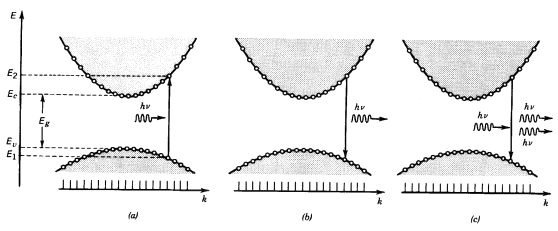
\includegraphics[width=0.6\linewidth]{BV-BC.png}
		\caption{\label{Img:Saleh-BV-BC}Esquema de bandas con las tres interacciones luz-materia en un semiconductor: (a) absorci\'on, (b) emisi\'on espont\'anea y (c) emisi\'on estimulada \cite{saleh2019fundamentals}.}
	\end{figure}

Debido a la poca intensidad de la emisi\'on espont\'anea, el proceso clave para los l\'aseres de semiconductor, al igual que para el resto, es el dominio de la emisi\'on estimulada. Si sobre el material con un electr\'on excitado en la banda de conducci\'on, se incide con un fot\'on de frecuencia $\nu_0$ igual a la diferencia de energ\'ias entre el estado excitado del electr\'on y el fundamental, se forzar\'a al electr\'on a decaer al nivel de menor energ\'ia. El fot\'on emitido en la recombinaci\'on del electr\'on tendr\'a las mismas propiedades que el fot\'on incidente, puediendo estos dos fotones interactuar con m\'as electrones excitados y as\'i producir la amplificaci\'on de la radiaci\'on incidente. Sin embargo, para que esta amplificaci\'on continue, debe haber una cantidad suficiente de electrones excitados. Para ello se utilizan fuentes de bombeo para obtener la inversi\'on de poblaci\'on.

El medio en el cu\'al se producen la mayor parte de emisiones espont\'aneas se denomina medio activo y para los l\'aseres de semiconductor suelen ser heteroestructuras por capas conuna uni\'on $pn$ en la direcci\'on de avance de la corriente. Cuando la corriente inyectada al l\'aser es suficientemente grande, se obtienen suficientes electrones en la banda de conducci\'on para amplificar la luz. Una ventaja de los l\'aseres de semiconductor es su alta densidad de electrones, que permiten alcanzar grandes valores para la ganancia y unas distancias pequeñas de la cavidad, del orden de $\sim 1$ mm.

La direcci\'on del medio activo con respecto al haz de luz emitido permite diferenciar entre dos tipos de l\'aseres de semiconductor. Los l\'aseres de emisi\'on vertical (VCSEL) presentan el medio activo ortogonal al haz de luz mientras que para los de emisión lateral el medio activo es paralelo al haz de luz emitida. 

NO SE SI HE DE MENCIONAR ALGO SOBRE LASERES DE MODO DISCRETO


	\addtocontents{toc}{\vspace{0.01cm}}
	\section{Procesos Estocásticos}
		\label{Intr:PrcsEstcs}
		
		
	%En esta seccion se va a hablar de los procesos estocasticos del problema y de las ecuaciones diferenciales estocasticas, asi como de su resolucion.
	

Los procesos estoc\'asticos permiten describir la evoluci\'on temporal de un sistema con comportamiento aleatorio a partir de la probabilidad estad\'istica de \'este \cite{gardiner1985handbook}. El ejemplo m\'as relevante de los procesos estoc\'asticos es el movimiento Browniano, que describe la evoluci\'on de la posici\'on de una part\'icula en el seno de un fluido, con impactos frecuentes e irregulares (aleatorios) con las part\'iculas del fluido. El movimiento Browniano viene definido por la ecuaci\'on de Langevin y as\'i, se puede describir su evoluci\'on realizando el promedio con diferentes perturbaciones aleatorias. Para el caso de un experimento esto equivaldr\'ia a realizar el promedio de los resultados, repitiendo el experimento un n\'umero suficiente de veces, hasta obtener la distribuci\'on de probabilidad del proceso.  Una forma alternativa de resoluci\'on del movimiento Browniano es a partir de la ecuaci\'on de Fokker-Planck. Para la evolución unidimensional esta ecuación es la ecuacion de difusión \ref{eq:Fokker-Plank} que da la probabilidad de que la posición de la partícula, $\overline{\underline{X}}(t)$, esté en $x$ en un tiempo $t$ con $P = P(x, t)$, donde $D$ es el coeficiente de difusión.

	\begin{equation}
		\frac{\partial P}{\partial t} = D \frac{\partial^2 P}{\partial x^2}
		\label{eq:Fokker-Plank}
	\end{equation}

	Otro ejemplo de proceso estoc\'astico es el de luz emitida por un l\'aser, cuya principal fuente de aleatoriedad viene dada por la emisión espontánea. Cuando la distribuci\'on de probabilidad del sistema para un conjunto de variables, no varia para un desplazamiento en el tiempo, se dice que se trata de un proceso estoc\'astico estacionario y se cumple que:
	
	\begin{equation}
		\begin{matrix}
			P(x_1, t_1,..., x_n, t_n) = P(x_1, t_1+\delta t,..., x_n, t_n+\delta t) \\ \\
			P(x_1, t_1, x_2, t_2) = P(x_1, x_2, \tau) \rightarrow \textrm{      con    } \tau = t_2 - t_1
		\end{matrix}
	\end{equation}



As\'i, la autocorrelaci\'on $R(t_1, t_2) = E\left[\overline{\underline{X}}(t_1)\overline{\underline{X}}(t_2)\right] = R_\tau$ depende solo de la diferencia de tiempos $\tau = t_1 - t_2$. En la ecuación anterior $E\left[\overline{\underline{X}}(t_1)\overline{\underline{X}}(t_2)\right]$ es el valor medio del producto de $\overline{\underline{X}}(t_1)$ por $\overline{\underline{X}}(t_2)$ sobre distintos resultados del experimento. Para un proceso estacionario, para el que la media es contante respecto a $t$, se puede relacionar la autocorrelaci\'on y el espectro de potencia $S(\omega)$ mediante el teorema de Kintchine, y la transformada de Fourier.

	\begin{equation}
		\begin{matrix}
			S(\omega) = \int_{-\infty }^{\infty } R(\tau) e^{-i\omega\tau} \mathrm{d} \tau \\ \\
			S(\omega) = \lim_{T \rightarrow 0} E\left[\frac{1}{2T} \left| \int_{-T }^{T} \overline{\underline{X}}(t) e^{-i\omega t} \mathrm{d} t \right| ^2 \right ]
		\end{matrix}
		\label{eq:kintchine}
	\end{equation}

%En los procesos estoc\'asticos Markovianos las probabilidades condicionadas est\'an determinadas por el conocimiento del pasado m\'as reciente , pues $\tau_1 \geq \tau_2 \geq \textrm{...} \geq \tau_n$. Para que un proceso estoc\'astico sea Markoviano ha de cumplir las condiciones de \ref{eq:Markiviano}, pudiendo obtener la ecuaci\'on de Chapman Kolmog\'orov \ref{eq:Ch-Kgr}.

	%\begin{equation}
	%	\begin{matrix}
	%		P(x_1, t_1, x_2, t_2, ...| y_1, \tau_1, y_2, \tau_2, ...) = P(x_1, t_1, x_2, t_2, ...| y_1, \tau_1) \\ \\
	%		P(x_1, t_1, x_2, t_2, ..., x_n, t_n) = P(x_1, t_1|x_2, t_2)P(x_2, t_2|x_3, t_3)...P(x_n-1, t_n-1|x_n, t_n)P(x_n, t_n)
	%	\end{matrix}
	%	\label{eq:Markiviano}	
	%\end{equation}

	%\begin{equation}
	%	P(x_1, t_1|x_3, t_3) = \int \mathrm{d}x_2 P(x_1, t_1|x_2, t_2)P(x_2, t_2|x_3, t_3)
	%	\label{eq:Ch-Kgr}
	%\end{equation}

Hay un tipo especial de procesos estocásticos en los que las probabilidades condicionadas están determinadas por el conocimiento del pasado más reciente, los procesos Markovianos. Para ellos la densidad de probabilidad de que el proceso tome el valor $z$ en $t$, sabiendo que tomó el valor $y$ en $t'$ ($P(z, t| y, t')$), satisface la ecuaci\'on de Fokker Plank \ref{eq:FPE}.

	\begin{equation}
		\frac{\partial P(z, t|y, t'))}{\partial t} = \frac{\partial }{\partial z}\left(A(z, t)P(z, t|y, t') \right ) + \frac{1}{2} \frac{\partial^2 }{\partial z^2}\left(B(z, t)P(z, t|y, t') \right )	
		\label{eq:FPE}
	\end{equation}

Un desarrollo de la ecuaci\'on \ref{eq:FPE} con condición inicial $P(z, t|y, t) = \delta(z-y)$ permite hallar una densidad de probabilidad $P(z, t+\Delta t | y, t)$ gaussiana con media $y(t) + A(y, t)\Delta t$ y varianza $B\Delta t$.

	\begin{equation}
		Z(t+\Delta t) = y(t) + A(y, t)\Delta t + \eta(t) \sqrt{\Delta t}
	\end{equation}

El sistema evoluciona con un arrastre sistem\'atico $y(t) + A(y, t)\Delta t$ sobre el que se superpone la fluctuaci\'on $\eta(t)$, gaussiana de media cero y varianza $B$.

Las ecuaciones diferenciales estoc\'asticas vienen definidas por la ecuaci\'on de Langevin de la forma:

	\begin{equation}
		\frac{\mathrm{d} x}{\mathrm{d} t} = a(x, t) + b(x, t) \xi(t)
		\label{eq:SDE}
	\end{equation}

En la ecuaci\'on \ref{eq:SDE} aparece el t\'ermino aleatorio $\xi(t)$ que describe la fluctuaci\'on r\'apida e irregular, con $\left \langle \xi(t) \right \rangle \equiv 0$ y $\left \langle \xi(t)\xi(t') \right \rangle = \delta(t-t')$. A este t\'ermino se le conoce como ruido blanco, debido a que se obtiene que el espectro de potencia es $S(\omega) = 1$ seg\'un la ecuaci\'on \ref{eq:kintchine} para $R(\tau) = \left \langle \xi(t)\xi(t') \right \rangle$.

Se obtiene que las ecuaciones \ref{eq:FPE} y \ref{eq:SDE} son equivalentes, por lo que se pueden simular procesos estoc\'asticos mediante la resoluci\'on num\'erica de \ref{eq:FPE} o mediante la integraci\'on num\'erica de la ecuaci\'on diferencial estoc\'astica \ref{eq:SDE}. 

Para la integraci\'on num\'erica de la ecuaci\'on estoc\'astica \ref{eq:SDE} se ha utilizado el algoritmo de Euler, discretizando el valor de $t$ (d$t \approx \Delta t$) y que d$x \approx x(t+\Delta t) - x(t)$. Considerando estas aproximaciones y teniendo en cuenta su equivalencia con la ecuaci\'on \ref{eq:FPE} se ha obtenido la siguiente expresi\'on:

	\begin{equation}
		\begin{matrix}
		x(t+\Delta t) = x(t) + a(x, t)\Delta t + \eta(t)\sqrt{\Delta t} \\ \\
		\eta(t) \textrm{ Gaussiano} \rightarrow \eta = \sqrt{V[\eta]} Z + E[\eta] = bZ
		\end{matrix}
		\label{eq:Gauss}
	\end{equation}

En la ecuaci\'on \ref{eq:Gauss} se muestran los t\'erminos del ruido gaussiano, siendo $E[\eta] = 0$ su media, $V[\eta] = b^2$ la varianza y $Z_i = N(0, 1)$ una distribuci\'on de probabilidad gaussiana. De esta forma, la soluci\'on a la ecuaci\'on \ref{eq:SDE}, considerando $x_i = x(t_i)$, queda \cite{gardiner1985handbook}:

	\begin{equation}
		x_{i+1} = x_i + a(x_i, t_i)\Delta t + b(x_i, t_i) Z_i\sqrt{\Delta t}
	\end{equation}


	\addtocontents{toc}{\vspace{0.01cm}}
	\section{Dinámica No Lineal}
		\label{Intr:NonLnr}
		
		
\section{Dinamica No lineal}

	En esta seccion se hablara de la dinamica no lineal, bifurcaciones, M.T., y de las dos formas de las que se puede obtener dinamica no lineal en nuestro laser de semiconductor

	\cite{rosado2018experimental}


	\addtocontents{toc}{\vspace{0.01cm}}
	\section{Peines de Frecuencia Óptica}
		\label{Intr:OFC}
		
		
Que son, caracteristicas principales y como se generan,...

	\subsection{\textit{Gain-Switching}}

		hola que tal todos

	\subsection{Inyección Ópticar}

		adios a todos 

	\subsection{Aplicaciones}




	%\addtocontents{toc}{\vspace{0.01cm}}
	%\section{Objetivo del Estudio}
	%	\label{Intr:Obj}
		
		%\input{}


			\addtocontents{toc}{\vspace{0.01cm}}
			\chapter{Láser en solitario}
				\label{Sol}

				El uso de dispositivos el\'ectricos de semiconductor supuso un avance enorme en la tecnolog\'ia, permitiendo desarrollar dispositivos m\'as eficientes y pequeños, conviertiendose en una parte fundamental de nuestra sociedad. Uno de estos dispositivos que han supuesto un gran avance son los l\'aseres de semiconductor, que ha descubierto un enorme campo de estudio, debido a sus importantes propiedades y a la multitud de aplicaciones en diferentes \'areas.

Este trabajo se centra en la creaci\'on de peines de frecuencia \'optica (OFC de sus siglas en ingl\'es) en un l\'aser de semiconductor de emisi\'on lateeral y modo discreto. Estos OFC presentan caracter\'isticas diversas en funci\'on de los par\'ametros que defienen su proceso de creaci\'on, debido a la din\'amica no lineal del sistema del l\'aser.

El objetivo de este trabajo es el estudio computacional del comportamiento de la diferentes regiones din\'amicas de los peines de frecuencia \'optica en l\'aseres de semiconductor con \gs\ e inyecci\'on \'optica. Este estudio permitir\'a entender los procesis f\'isicos relevantes en la formaci\'on de los OFC.

En este cap\'itulo se han introducido los conceptos te\'oricos relevantes de los temas tratados en este trabajo. Se ha realizado una breve introducci\'on sobre los l\'aseres de semiconductor, los procesos estoc\'asticos y la din\'amica no lineal, pasando a continuaci\'on a describir los peines de frecuencia \'optica y dos de los m\'etodos utilizados para su obtenci\'on: el \gs\ y la inyecci\'on \'optica.

	\addtocontents{toc}{\vspace{0.01cm}}
	\section{Láseres de Semiconductor}
		\label{Intr:LsrSmcdtr}
		
		\graphicspath{{./Introduccion/Figures/}}

La caracter\'istica principal de los semiconductores es la separaci\'on o gap entre la banda de valencia y la banda de conducci\'on, con un valor pequeño ($\varepsilon_g  = \varepsilon_C - \varepsilon_V \sim 0.1 - 3$ eV). Al tener un gap pequeño pueden darse saltos entre electrones de la banda de valencia y la banda de conducci\'on, apartir de la mediaci\'on de un fot\'on. Estas interacciones solo se pueden dar para energias del fot\'on $h\nu > \varepsilon_g$.

Las tres posibles formas de interacci\'on luz-materia son la emisi\'on espont\'anea, la emisi\'on estimulada y la absorci\'on. En un material semiconductor a $T = 0$K se tiene la banda de valencia completamente llena y la banda de conducci\'on vac\'ia. Al aumentar la temperatura se pueden dar saltos de los electrones a la banda de conducci\'on debido al pequeño gap. Al situarse un electr\'on en un nivel superior de energ\'ia, \'este tender\'a a volver a su estado de m\'inima energ\'ia recombinandose de nuevo en la banda de valencia, pudiendo emitir un fot\'on en el proceso. Este proceso es el denominado emisi\'on espont\'anea y es muy d\'ebil debido a que cada fot\'on puede tener diferente fase y direcci\'on.

	\begin{figure}[H]
		\centering
		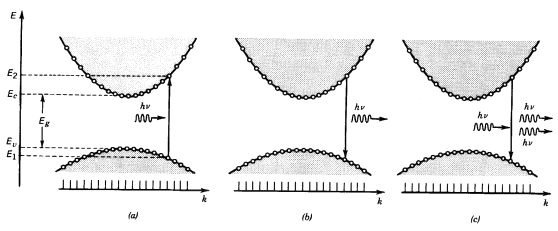
\includegraphics[width=0.6\linewidth]{BV-BC.png}
		\caption{\label{Img:Saleh-BV-BC}Esquema de bandas con las tres interacciones luz-materia en un semiconductor: (a) absorci\'on, (b) emisi\'on espont\'anea y (c) emisi\'on estimulada \cite{saleh2019fundamentals}.}
	\end{figure}

Debido a la poca intensidad de la emisi\'on espont\'anea, el proceso clave para los l\'aseres de semiconductor, al igual que para el resto, es el dominio de la emisi\'on estimulada. Si sobre el material con un electr\'on excitado en la banda de conducci\'on, se incide con un fot\'on de frecuencia $\nu_0$ igual a la diferencia de energ\'ias entre el estado excitado del electr\'on y el fundamental, se forzar\'a al electr\'on a decaer al nivel de menor energ\'ia. El fot\'on emitido en la recombinaci\'on del electr\'on tendr\'a las mismas propiedades que el fot\'on incidente, puediendo estos dos fotones interactuar con m\'as electrones excitados y as\'i producir la amplificaci\'on de la radiaci\'on incidente. Sin embargo, para que esta amplificaci\'on continue, debe haber una cantidad suficiente de electrones excitados. Para ello se utilizan fuentes de bombeo para obtener la inversi\'on de poblaci\'on.

El medio en el cu\'al se producen la mayor parte de emisiones espont\'aneas se denomina medio activo y para los l\'aseres de semiconductor suelen ser heteroestructuras por capas conuna uni\'on $pn$ en la direcci\'on de avance de la corriente. Cuando la corriente inyectada al l\'aser es suficientemente grande, se obtienen suficientes electrones en la banda de conducci\'on para amplificar la luz. Una ventaja de los l\'aseres de semiconductor es su alta densidad de electrones, que permiten alcanzar grandes valores para la ganancia y unas distancias pequeñas de la cavidad, del orden de $\sim 1$ mm.

La direcci\'on del medio activo con respecto al haz de luz emitido permite diferenciar entre dos tipos de l\'aseres de semiconductor. Los l\'aseres de emisi\'on vertical (VCSEL) presentan el medio activo ortogonal al haz de luz mientras que para los de emisión lateral el medio activo es paralelo al haz de luz emitida. 

NO SE SI HE DE MENCIONAR ALGO SOBRE LASERES DE MODO DISCRETO


	\addtocontents{toc}{\vspace{0.01cm}}
	\section{Procesos Estocásticos}
		\label{Intr:PrcsEstcs}
		
		
	%En esta seccion se va a hablar de los procesos estocasticos del problema y de las ecuaciones diferenciales estocasticas, asi como de su resolucion.
	

Los procesos estoc\'asticos permiten describir la evoluci\'on temporal de un sistema con comportamiento aleatorio a partir de la probabilidad estad\'istica de \'este \cite{gardiner1985handbook}. El ejemplo m\'as relevante de los procesos estoc\'asticos es el movimiento Browniano, que describe la evoluci\'on de la posici\'on de una part\'icula en el seno de un fluido, con impactos frecuentes e irregulares (aleatorios) con las part\'iculas del fluido. El movimiento Browniano viene definido por la ecuaci\'on de Langevin y as\'i, se puede describir su evoluci\'on realizando el promedio con diferentes perturbaciones aleatorias. Para el caso de un experimento esto equivaldr\'ia a realizar el promedio de los resultados, repitiendo el experimento un n\'umero suficiente de veces, hasta obtener la distribuci\'on de probabilidad del proceso.  Una forma alternativa de resoluci\'on del movimiento Browniano es a partir de la ecuaci\'on de Fokker-Planck. Para la evolución unidimensional esta ecuación es la ecuacion de difusión \ref{eq:Fokker-Plank} que da la probabilidad de que la posición de la partícula, $\overline{\underline{X}}(t)$, esté en $x$ en un tiempo $t$ con $P = P(x, t)$, donde $D$ es el coeficiente de difusión.

	\begin{equation}
		\frac{\partial P}{\partial t} = D \frac{\partial^2 P}{\partial x^2}
		\label{eq:Fokker-Plank}
	\end{equation}

	Otro ejemplo de proceso estoc\'astico es el de luz emitida por un l\'aser, cuya principal fuente de aleatoriedad viene dada por la emisión espontánea. Cuando la distribuci\'on de probabilidad del sistema para un conjunto de variables, no varia para un desplazamiento en el tiempo, se dice que se trata de un proceso estoc\'astico estacionario y se cumple que:
	
	\begin{equation}
		\begin{matrix}
			P(x_1, t_1,..., x_n, t_n) = P(x_1, t_1+\delta t,..., x_n, t_n+\delta t) \\ \\
			P(x_1, t_1, x_2, t_2) = P(x_1, x_2, \tau) \rightarrow \textrm{      con    } \tau = t_2 - t_1
		\end{matrix}
	\end{equation}



As\'i, la autocorrelaci\'on $R(t_1, t_2) = E\left[\overline{\underline{X}}(t_1)\overline{\underline{X}}(t_2)\right] = R_\tau$ depende solo de la diferencia de tiempos $\tau = t_1 - t_2$. En la ecuación anterior $E\left[\overline{\underline{X}}(t_1)\overline{\underline{X}}(t_2)\right]$ es el valor medio del producto de $\overline{\underline{X}}(t_1)$ por $\overline{\underline{X}}(t_2)$ sobre distintos resultados del experimento. Para un proceso estacionario, para el que la media es contante respecto a $t$, se puede relacionar la autocorrelaci\'on y el espectro de potencia $S(\omega)$ mediante el teorema de Kintchine, y la transformada de Fourier.

	\begin{equation}
		\begin{matrix}
			S(\omega) = \int_{-\infty }^{\infty } R(\tau) e^{-i\omega\tau} \mathrm{d} \tau \\ \\
			S(\omega) = \lim_{T \rightarrow 0} E\left[\frac{1}{2T} \left| \int_{-T }^{T} \overline{\underline{X}}(t) e^{-i\omega t} \mathrm{d} t \right| ^2 \right ]
		\end{matrix}
		\label{eq:kintchine}
	\end{equation}

%En los procesos estoc\'asticos Markovianos las probabilidades condicionadas est\'an determinadas por el conocimiento del pasado m\'as reciente , pues $\tau_1 \geq \tau_2 \geq \textrm{...} \geq \tau_n$. Para que un proceso estoc\'astico sea Markoviano ha de cumplir las condiciones de \ref{eq:Markiviano}, pudiendo obtener la ecuaci\'on de Chapman Kolmog\'orov \ref{eq:Ch-Kgr}.

	%\begin{equation}
	%	\begin{matrix}
	%		P(x_1, t_1, x_2, t_2, ...| y_1, \tau_1, y_2, \tau_2, ...) = P(x_1, t_1, x_2, t_2, ...| y_1, \tau_1) \\ \\
	%		P(x_1, t_1, x_2, t_2, ..., x_n, t_n) = P(x_1, t_1|x_2, t_2)P(x_2, t_2|x_3, t_3)...P(x_n-1, t_n-1|x_n, t_n)P(x_n, t_n)
	%	\end{matrix}
	%	\label{eq:Markiviano}	
	%\end{equation}

	%\begin{equation}
	%	P(x_1, t_1|x_3, t_3) = \int \mathrm{d}x_2 P(x_1, t_1|x_2, t_2)P(x_2, t_2|x_3, t_3)
	%	\label{eq:Ch-Kgr}
	%\end{equation}

Hay un tipo especial de procesos estocásticos en los que las probabilidades condicionadas están determinadas por el conocimiento del pasado más reciente, los procesos Markovianos. Para ellos la densidad de probabilidad de que el proceso tome el valor $z$ en $t$, sabiendo que tomó el valor $y$ en $t'$ ($P(z, t| y, t')$), satisface la ecuaci\'on de Fokker Plank \ref{eq:FPE}.

	\begin{equation}
		\frac{\partial P(z, t|y, t'))}{\partial t} = \frac{\partial }{\partial z}\left(A(z, t)P(z, t|y, t') \right ) + \frac{1}{2} \frac{\partial^2 }{\partial z^2}\left(B(z, t)P(z, t|y, t') \right )	
		\label{eq:FPE}
	\end{equation}

Un desarrollo de la ecuaci\'on \ref{eq:FPE} con condición inicial $P(z, t|y, t) = \delta(z-y)$ permite hallar una densidad de probabilidad $P(z, t+\Delta t | y, t)$ gaussiana con media $y(t) + A(y, t)\Delta t$ y varianza $B\Delta t$.

	\begin{equation}
		Z(t+\Delta t) = y(t) + A(y, t)\Delta t + \eta(t) \sqrt{\Delta t}
	\end{equation}

El sistema evoluciona con un arrastre sistem\'atico $y(t) + A(y, t)\Delta t$ sobre el que se superpone la fluctuaci\'on $\eta(t)$, gaussiana de media cero y varianza $B$.

Las ecuaciones diferenciales estoc\'asticas vienen definidas por la ecuaci\'on de Langevin de la forma:

	\begin{equation}
		\frac{\mathrm{d} x}{\mathrm{d} t} = a(x, t) + b(x, t) \xi(t)
		\label{eq:SDE}
	\end{equation}

En la ecuaci\'on \ref{eq:SDE} aparece el t\'ermino aleatorio $\xi(t)$ que describe la fluctuaci\'on r\'apida e irregular, con $\left \langle \xi(t) \right \rangle \equiv 0$ y $\left \langle \xi(t)\xi(t') \right \rangle = \delta(t-t')$. A este t\'ermino se le conoce como ruido blanco, debido a que se obtiene que el espectro de potencia es $S(\omega) = 1$ seg\'un la ecuaci\'on \ref{eq:kintchine} para $R(\tau) = \left \langle \xi(t)\xi(t') \right \rangle$.

Se obtiene que las ecuaciones \ref{eq:FPE} y \ref{eq:SDE} son equivalentes, por lo que se pueden simular procesos estoc\'asticos mediante la resoluci\'on num\'erica de \ref{eq:FPE} o mediante la integraci\'on num\'erica de la ecuaci\'on diferencial estoc\'astica \ref{eq:SDE}. 

Para la integraci\'on num\'erica de la ecuaci\'on estoc\'astica \ref{eq:SDE} se ha utilizado el algoritmo de Euler, discretizando el valor de $t$ (d$t \approx \Delta t$) y que d$x \approx x(t+\Delta t) - x(t)$. Considerando estas aproximaciones y teniendo en cuenta su equivalencia con la ecuaci\'on \ref{eq:FPE} se ha obtenido la siguiente expresi\'on:

	\begin{equation}
		\begin{matrix}
		x(t+\Delta t) = x(t) + a(x, t)\Delta t + \eta(t)\sqrt{\Delta t} \\ \\
		\eta(t) \textrm{ Gaussiano} \rightarrow \eta = \sqrt{V[\eta]} Z + E[\eta] = bZ
		\end{matrix}
		\label{eq:Gauss}
	\end{equation}

En la ecuaci\'on \ref{eq:Gauss} se muestran los t\'erminos del ruido gaussiano, siendo $E[\eta] = 0$ su media, $V[\eta] = b^2$ la varianza y $Z_i = N(0, 1)$ una distribuci\'on de probabilidad gaussiana. De esta forma, la soluci\'on a la ecuaci\'on \ref{eq:SDE}, considerando $x_i = x(t_i)$, queda \cite{gardiner1985handbook}:

	\begin{equation}
		x_{i+1} = x_i + a(x_i, t_i)\Delta t + b(x_i, t_i) Z_i\sqrt{\Delta t}
	\end{equation}


	\addtocontents{toc}{\vspace{0.01cm}}
	\section{Dinámica No Lineal}
		\label{Intr:NonLnr}
		
		
\section{Dinamica No lineal}

	En esta seccion se hablara de la dinamica no lineal, bifurcaciones, M.T., y de las dos formas de las que se puede obtener dinamica no lineal en nuestro laser de semiconductor

	\cite{rosado2018experimental}


	\addtocontents{toc}{\vspace{0.01cm}}
	\section{Peines de Frecuencia Óptica}
		\label{Intr:OFC}
		
		
Que son, caracteristicas principales y como se generan,...

	\subsection{\textit{Gain-Switching}}

		hola que tal todos

	\subsection{Inyección Ópticar}

		adios a todos 

	\subsection{Aplicaciones}




	%\addtocontents{toc}{\vspace{0.01cm}}
	%\section{Objetivo del Estudio}
	%	\label{Intr:Obj}
		
		%\input{}
	

			\addtocontents{toc}{\vspace{0.01cm}}
			\chapter{Inyecci\'on Óptica}

				\graphicspath{{../Graphics/Cpt2-InjectCW/}}


			\begin{figure}[H]
				\centering
				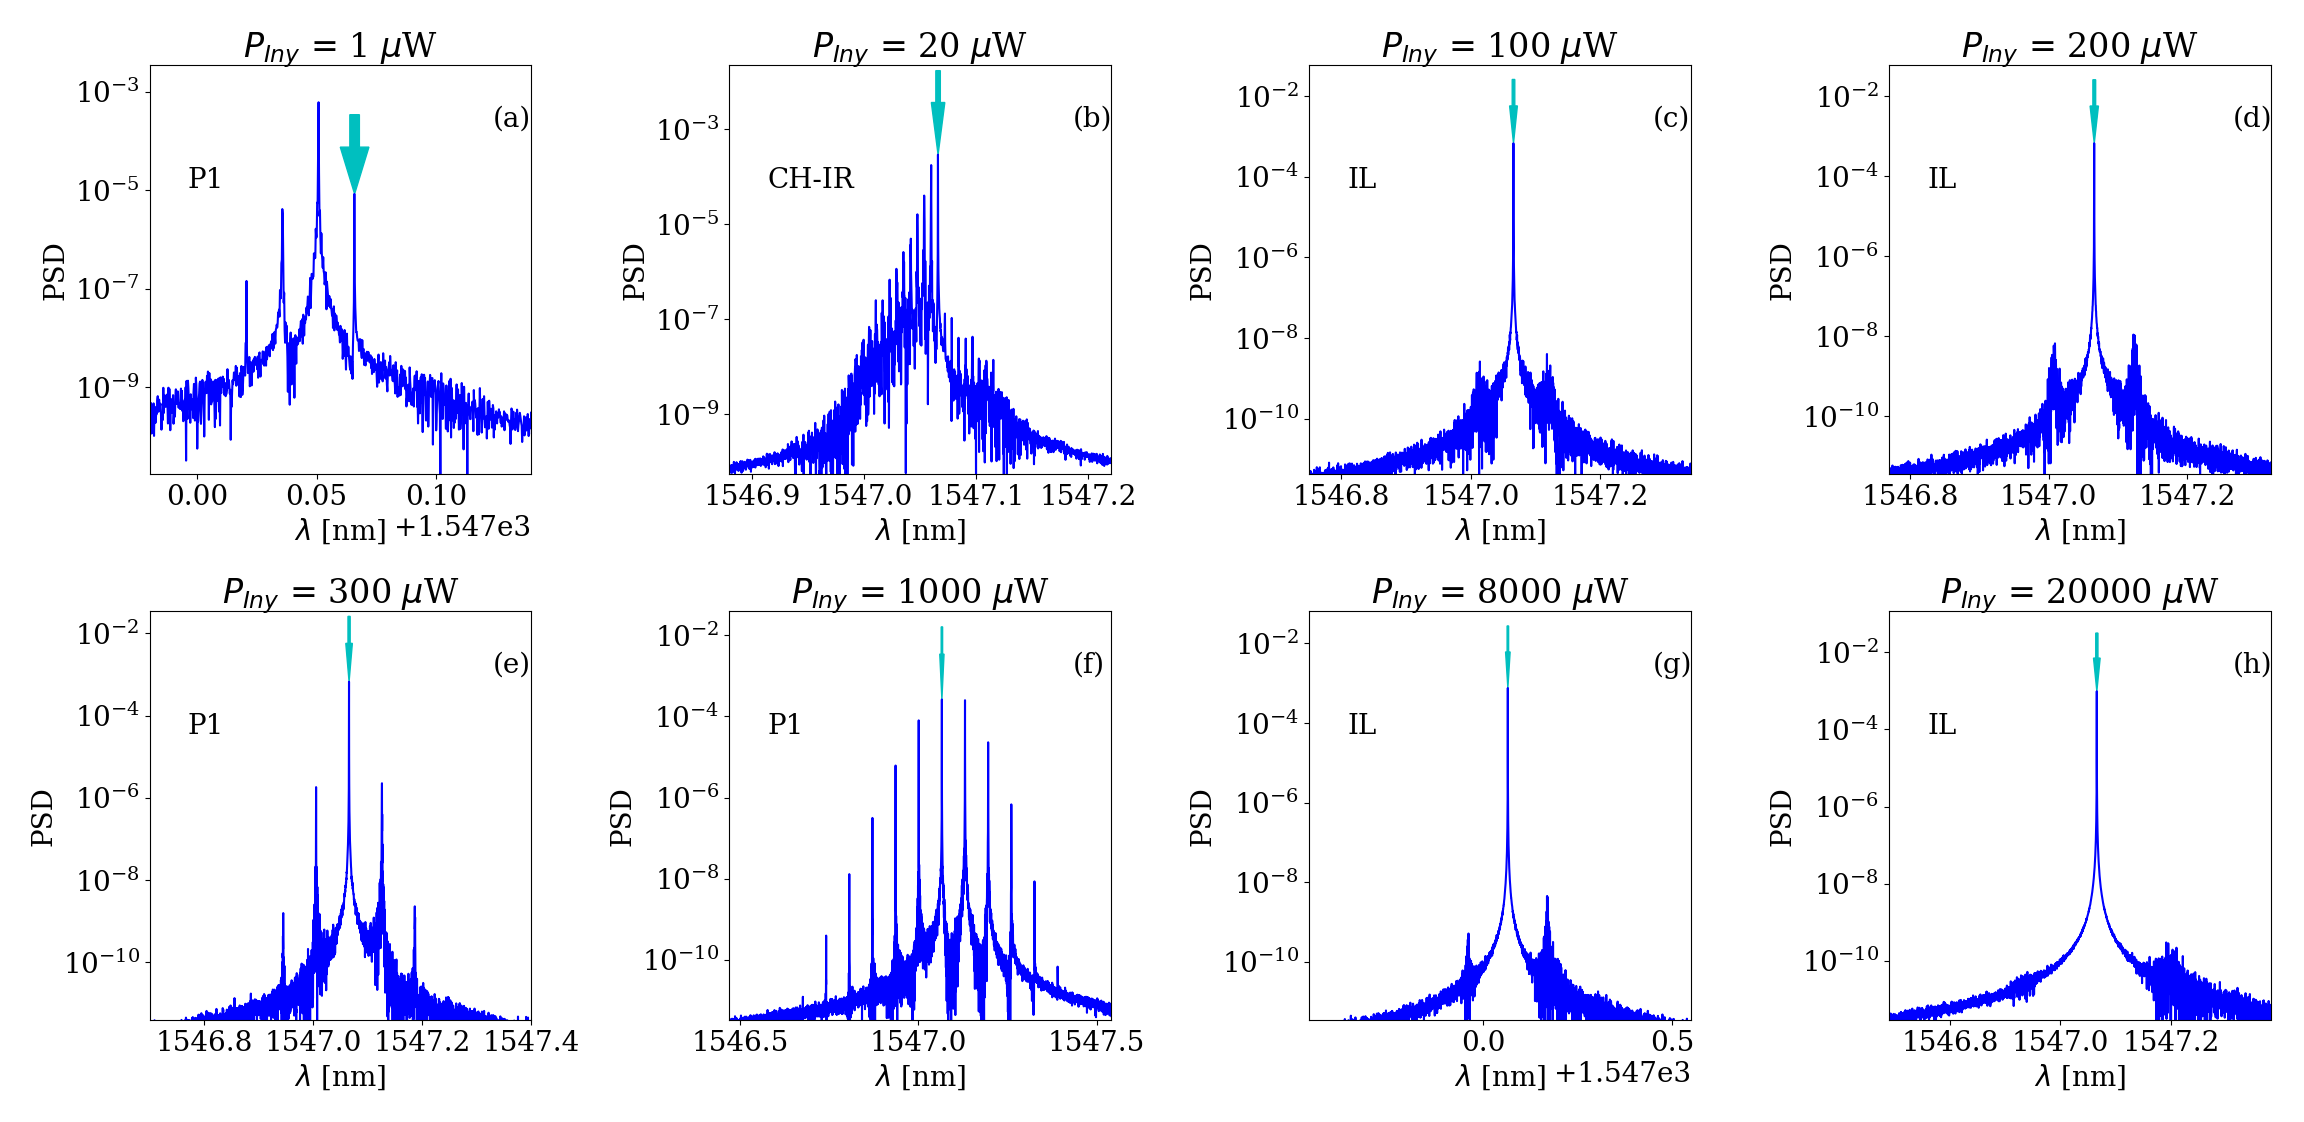
\includegraphics[width=1.0\linewidth]{zoneMap.png}
				\caption{\label{Img:widgets}el pie de pagina que le quieras 	poner a la imagen}
			\end{figure}

			\begin{figure}[H]
				\centering
				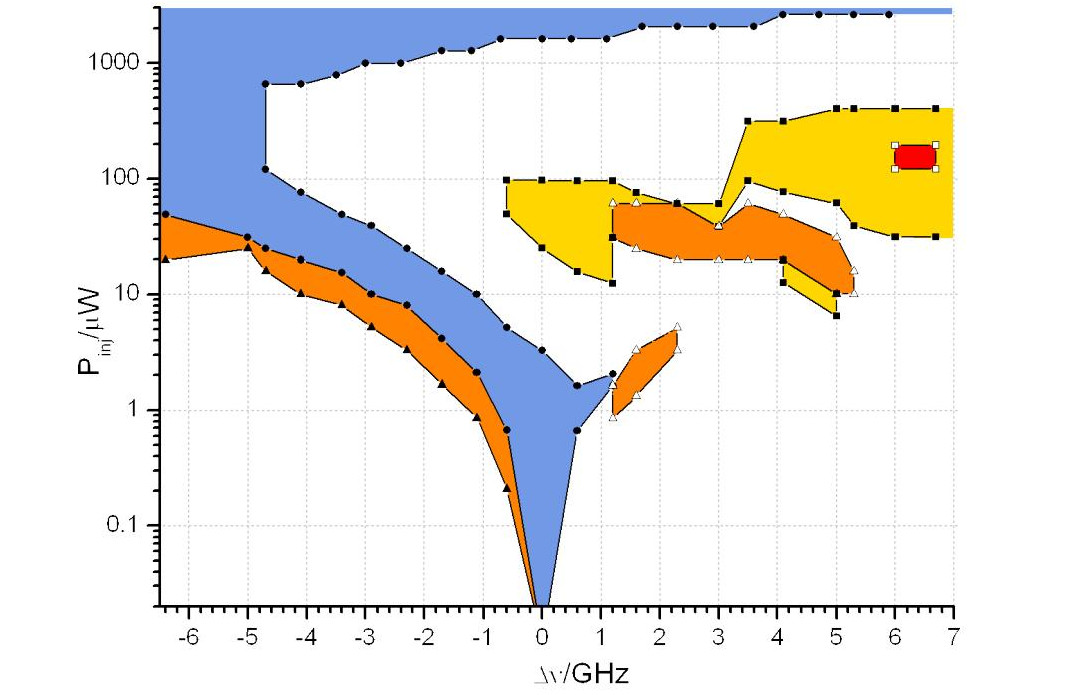
\includegraphics[width=1.0\linewidth]{mapa.jpg}
				\caption{\label{fig:map}Map}	
			\end{figure}

			\begin{figure}[H]
				\centering
				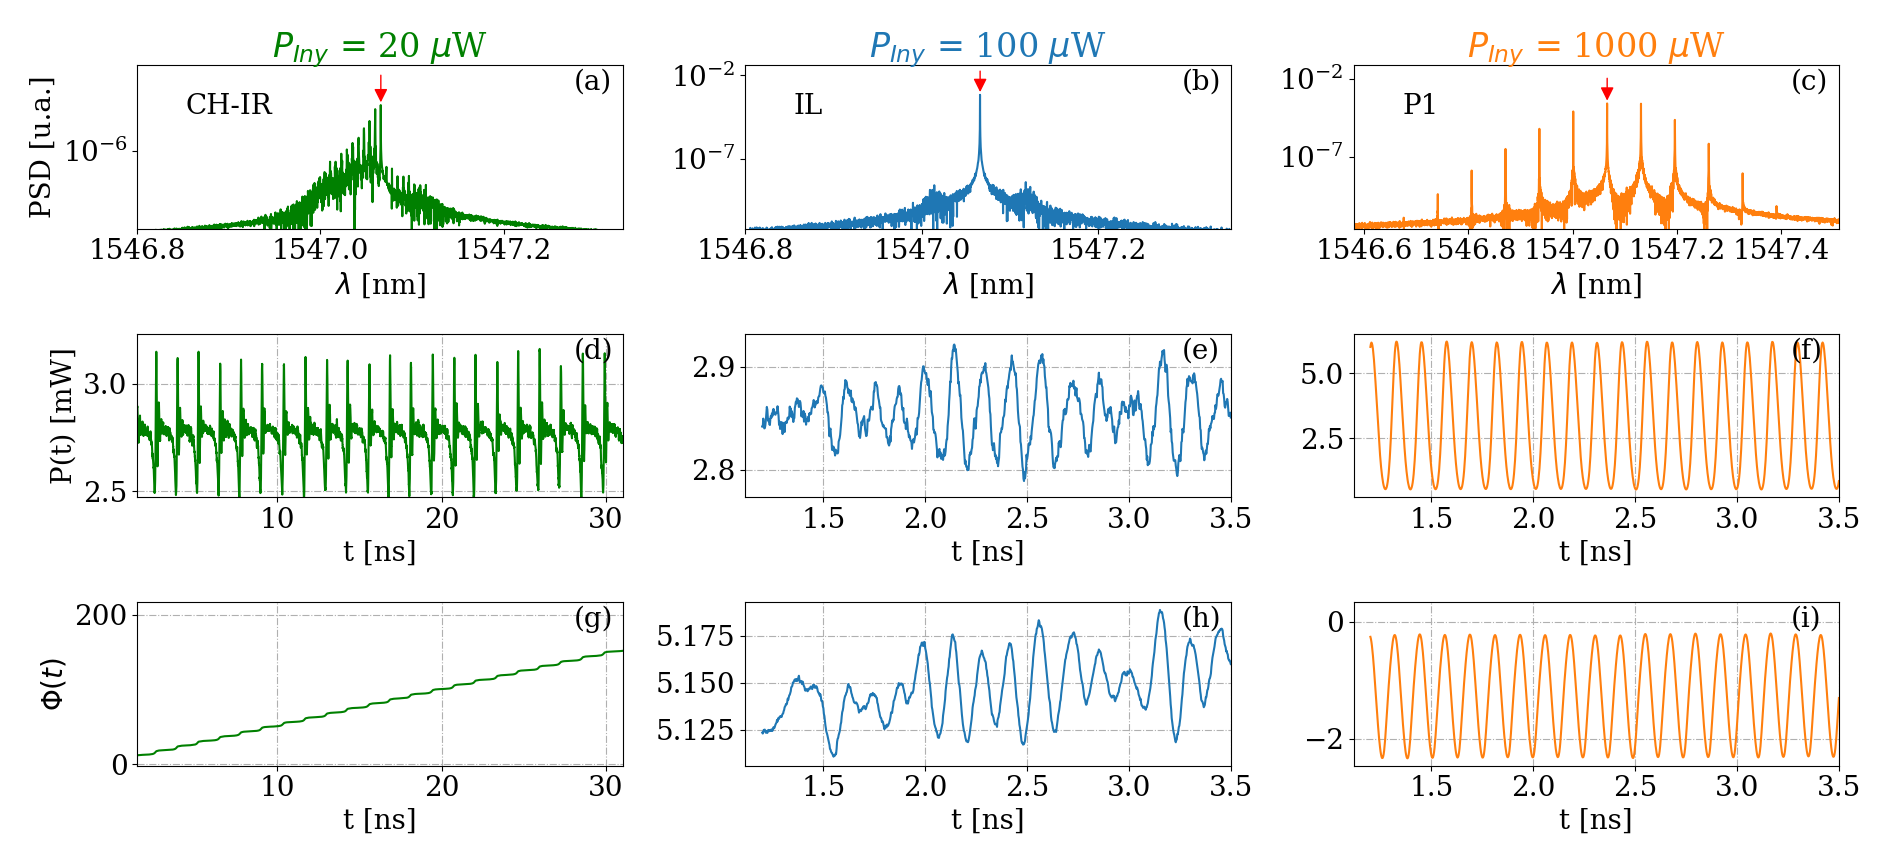
\includegraphics[width=1.0\linewidth]{zoneRtEq.png}
				\caption{\label{fig:zoneRtEq}ZoneRtEq}	
			\end{figure}

			\begin{figure}[H]
				\centering
				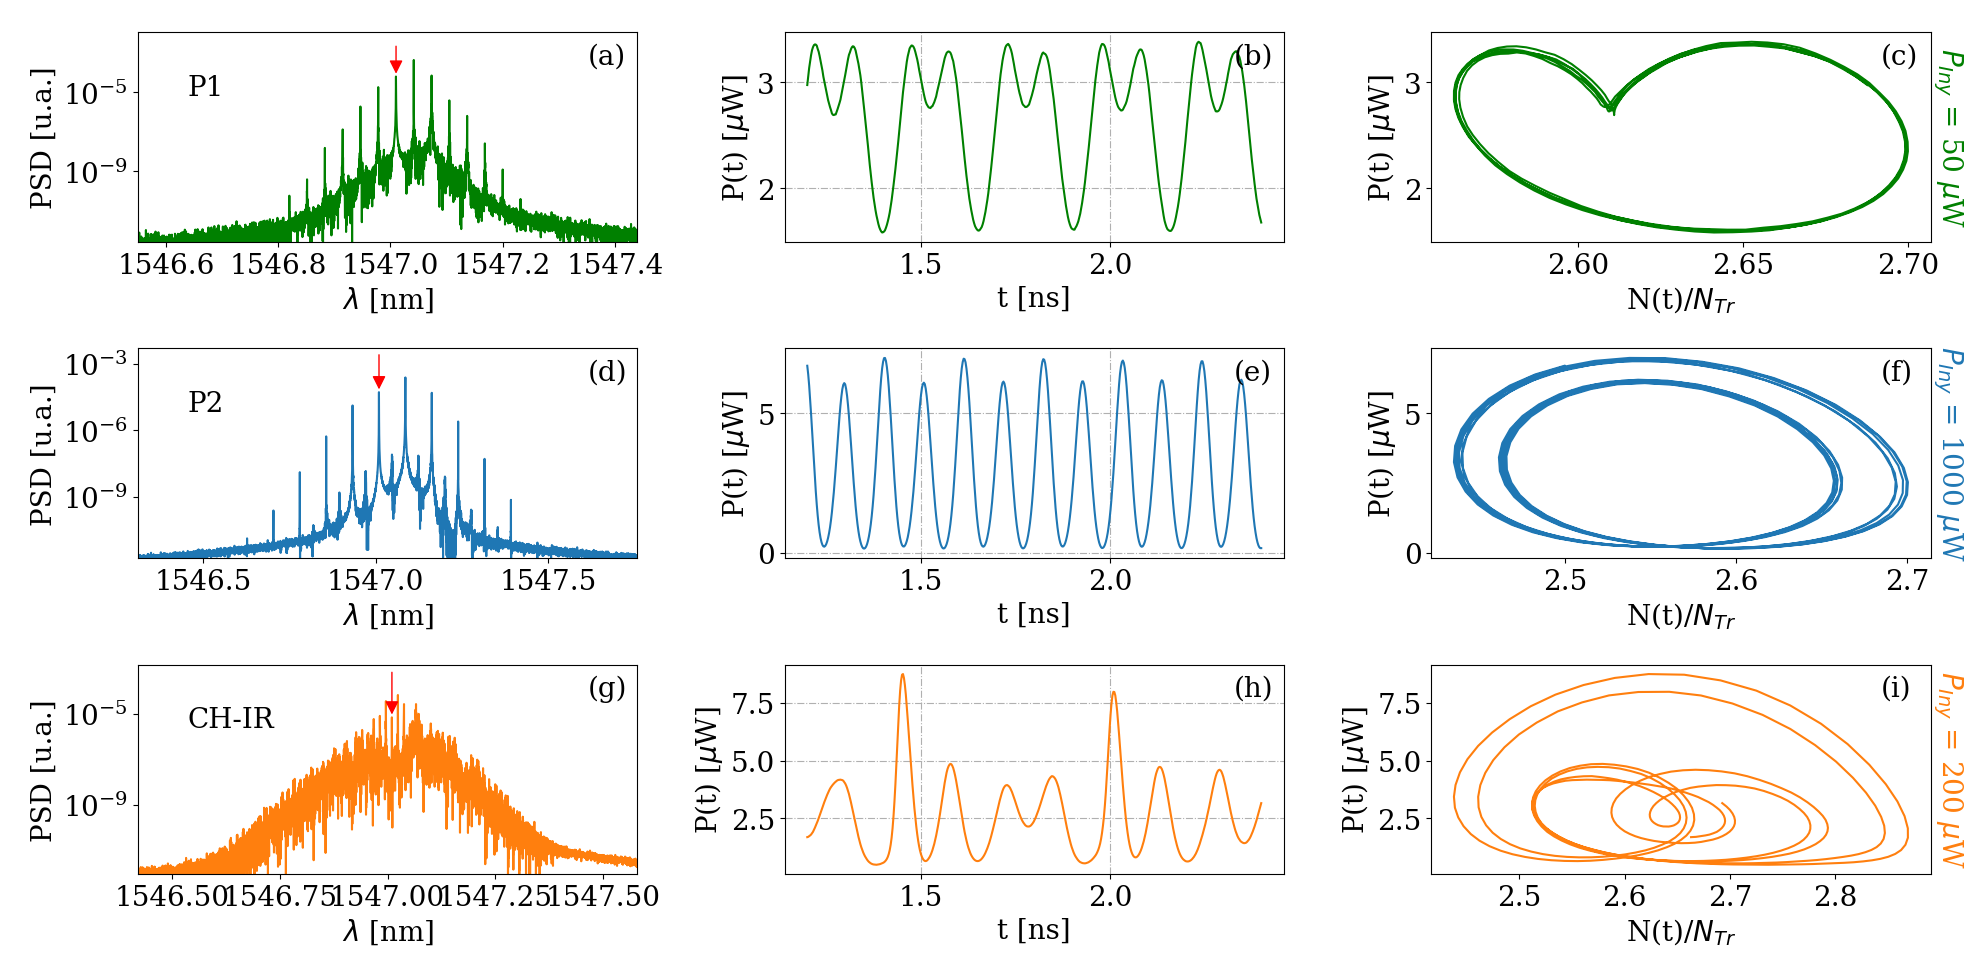
\includegraphics[width=1.0\linewidth]{P2zone.png}
				\caption{\label{fig:P2zone}P2zone}	
			\end{figure}


			\addtocontents{toc}{\vspace{0.01cm}}
			\chapter{Inyecci\'on Óptica en un láser \gs}

				\graphicspath{{../Graphics/Cpt3-CombInject/}}

En este cap\'itulo se han combinado los m\'etodos de generaci\'on de OFC estudiados en los cap\'itulos anteriores, abordando el estudio de los r\'egimenes din\'amicos que existen en la generaci\'on de OFC mediante \gs\ e inyecci\'on de luz. Se ha trabajado con el l\'aser ML con $\ibias = 35$ mA, $V_{RF} = 1.$ V y alta frecuencia $f_R = 5$ GHz. Para las condiciones de inyecci\'on de SL se ha tomado un \'unico valor de $\delta\nu = -2$ GHz, variando la potencia de inyecci\'on $P_{Iny}$.

En la Figura \ref{Img:MapGS-IO} se muestran los espectros \'opticos de las diferentes regiones din\'amicas obtenidas para distintas $P_{Iny}$ a $\delta\nu = -2$ GHz. 


			\begin{figure}[H]
				\centering
				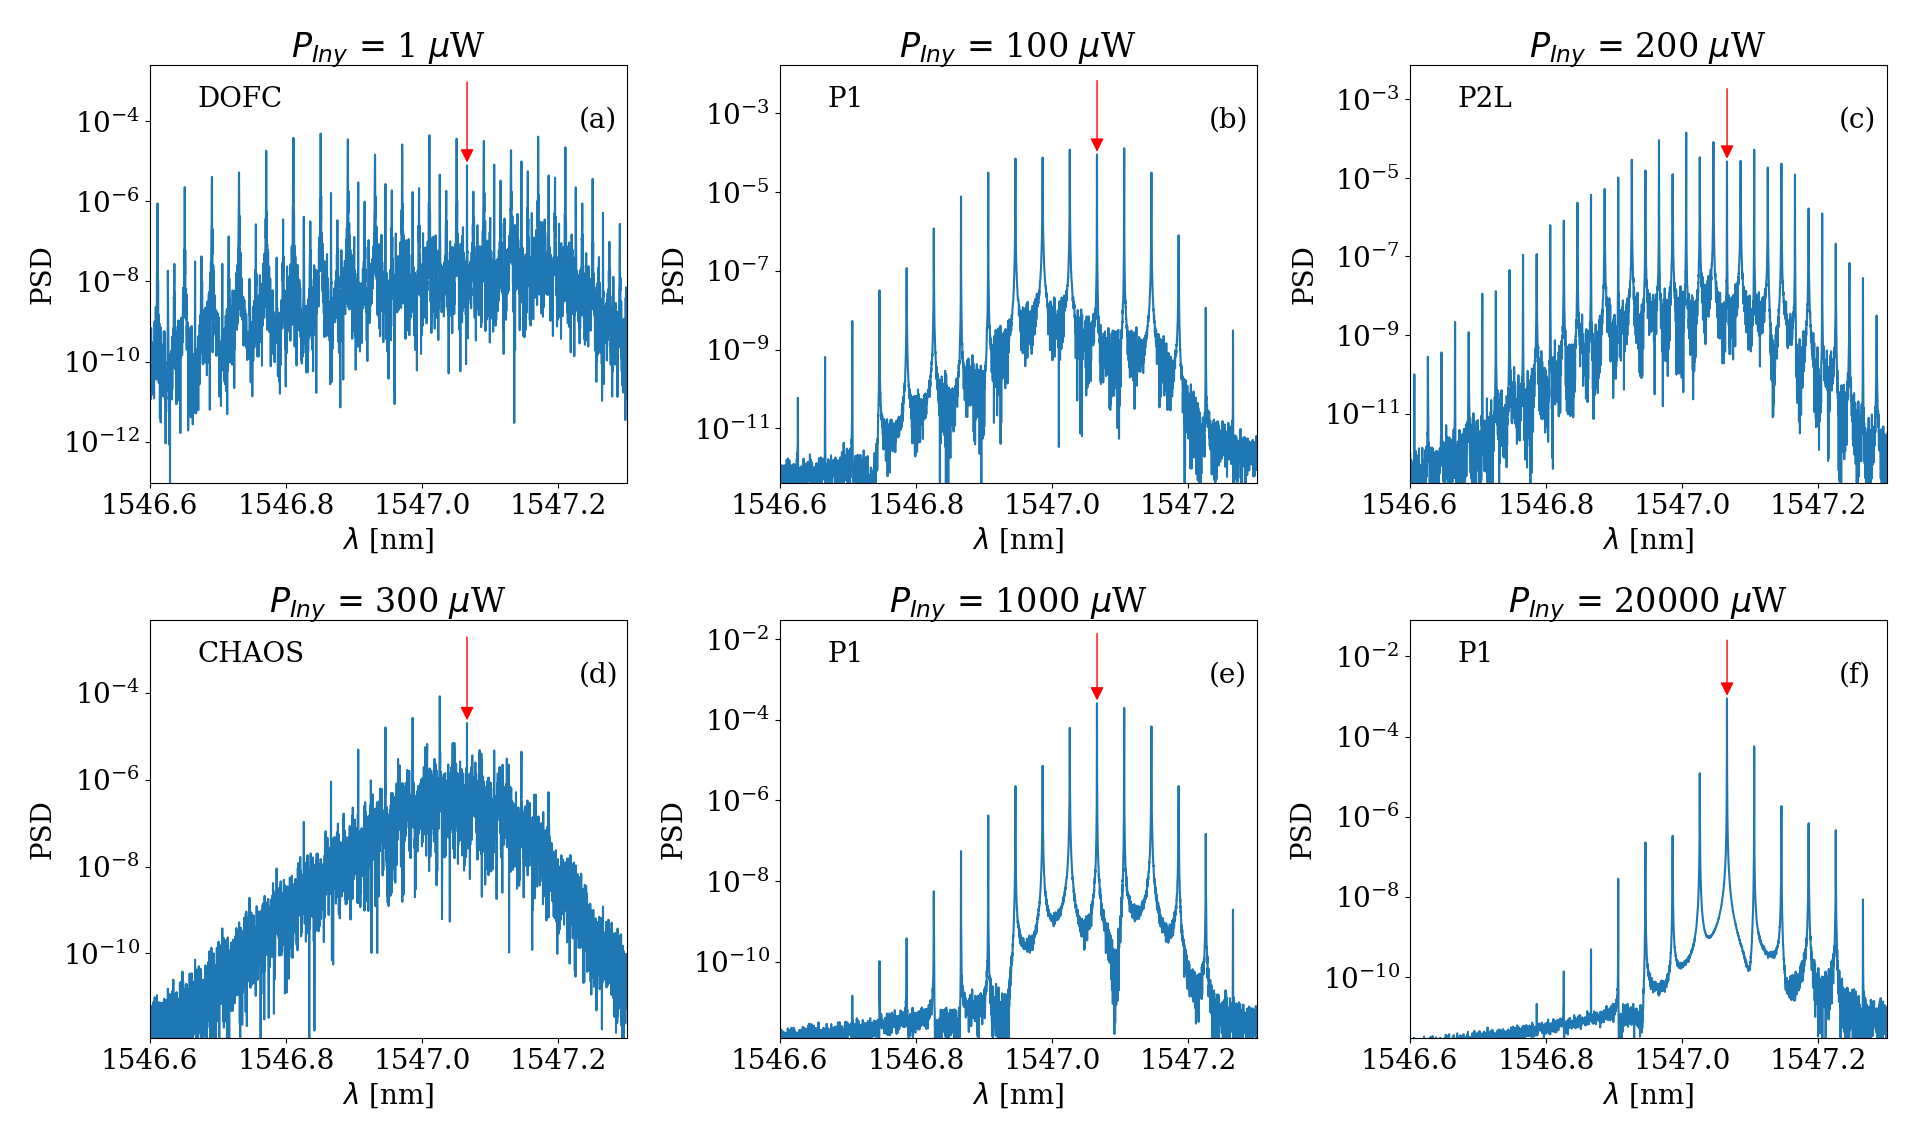
\includegraphics[width=1.0\linewidth]{psdMap.png}
				\caption{\label{Img:MapGS-IO}Espectros \'opticos obtenidos mediante \gs\ e inyección \'optica de las diferentes regiones dinámicas obtenidas para diferentes $P_{Iny}$ a $\delta\nu = -2$ GHz. Se indica la frecuencia de inyección $\nu_{SL}$ con una flecha y $P_{Iny}$ para cada espectro \'optico.}
			\end{figure}

		Para $P_{Iny} = 1\;\mu$W se obtiene un espectro \'optico con doble peine \'optico de frecuencias, DOFC, observando dos picos de emisión a cada lado del OFC principal (Figura \ref{Img:MapGS-IO} (a)). El DOFC se desruye al aumentar la potencia de inyección, obteniendo un OFC simple en la regi\'on P1 para $P_{Iny} = 100\;\mu$W (Figura \ref{Img:MapGS-IO} (b)). Al aumentar $P_{Iny} = 200 \;\mu$W se produce un doblamiento de periodo P2, obteniendo un OFC cuyas frecuencias de separaci\'on entre pico es la mitad que para la regi\'on P1 (Figura \ref{Img:MapGS-IO} (c)). La región de caos, CHAOS, se obtiene para $P_{Iny} = 300\;\mu$W, para la que el OFC se destruye (Figura \ref{Img:MapGS-IO} (d)). Con altas potencias de inyecci\'on $P_{Iny} = 1000\;\mu$W y $ 20000\;\mu$W se alcanza nuevamente la regi\'on P1 con un pico m\'aximo para la frecuencia de inyecci\'on $\nu_{SL}$. Dentro de esta regi\'on, al aumentar $P_{Iny}$ tanto el ruido debido a la emisi\'on espont\'anea como los picos de emisi\'on que se encuentran a los lados del pico en $\nu_{SL}$ disminuyen, mientras que el pico co nla frecuencia de inyecci\'on aumenta. Esta tendencia puede indicar la existencia de una nueva regi\'on con IL para $P_{Iny}$ superiores a los valores con los que se ha trabajado.

		Se han estudiado y comparado algunos casos concretos de las regiones mostradas en la Figura \ref{Img:MapGS-IO}, analizando el comportamiento de las variables internas con el objetivo de entender mejor los fen\'omenos que se producen en cada caso, de cara a realizar una correcta distinci\'on de las diferentes regiones din\'amicas.

		En la Figura \ref{fig:p1-p2} se muestran los espectros \'opticos, $P(t)$ y el atractor en el espacio de los estados de las ecuaciones de balance, despreciando los efectos de la fase \'optica; para $\delta\nu = -2$GHz y $P_{Iny} = 100\;\mu$W y $200\;\mu$W.

			\begin{figure}[H]
				\centering
				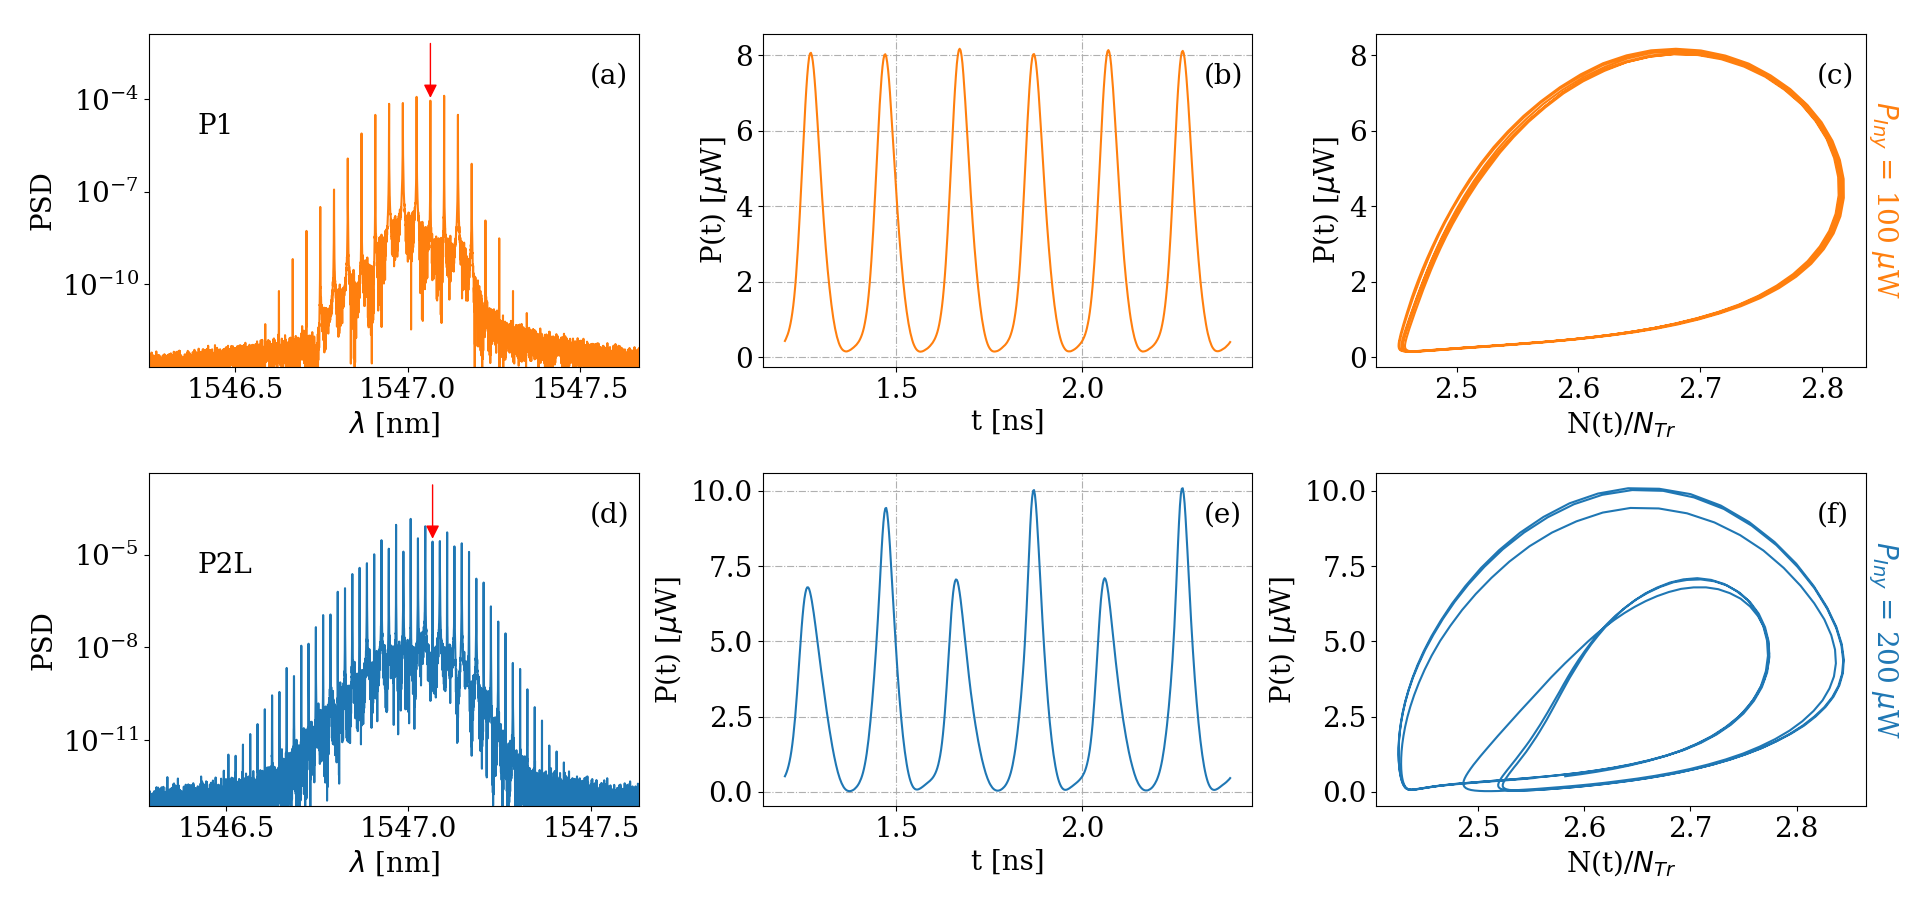
\includegraphics[width=1.0\linewidth]{p1-p2.png}
				\caption{\label{fig:p1-p2}Espectros \'opticos, $P(t)$ y atractor en el espacio de los estados de las ecuaciones de balance, despreciando los efectos de la fase \'optica; para $\delta\nu = -2$GHz y $P_{Iny} = 100\;\mu$W (P1, naranja) y $200\;\mu$W (P2, azul).}	
			\end{figure}

		Los resultados de la Figura \ref{fig:p1-p2} permiten comparar m\'s a fondo las regiones P1 y P2, obteniendo para ambos casos dos OFC con similares perfiles pero cuya separaci\'on entre l\'ineas es la mitad para el caso de P2. Esto se puede observar en la Figura \ref{fig:p1-p2} (e) en la que la diferencia de amplitudes entre picos continuos produce que el periodo de las oscilaciones de $P(t)$ no sea el tiempo entre picos continuas, sino el tiempo entre picos con la misma amplitud, que es el doble. Tambi\'en se puede observar en la Figura \ref{fig:p1-p2} (f) en la que se obtiene una doble oscilación con un diagrama similar al de la Figura \ref{fig:P2zon} (f) para la regi\'on P2 del c\'apitulo anterior.

		En la Figura \ref{fig:chaos} se muestran los espectros \'opticos, $P(t)$ y el atractor en el espacio de los estados de las ecuaciones de balance, despreciando los efectos de la fase \'optica; para $\delta\nu = -2$GHz y $P_{Iny} = 1\;\mu$W y $300\;\mu$W.

			\begin{figure}[H]
				\centering
				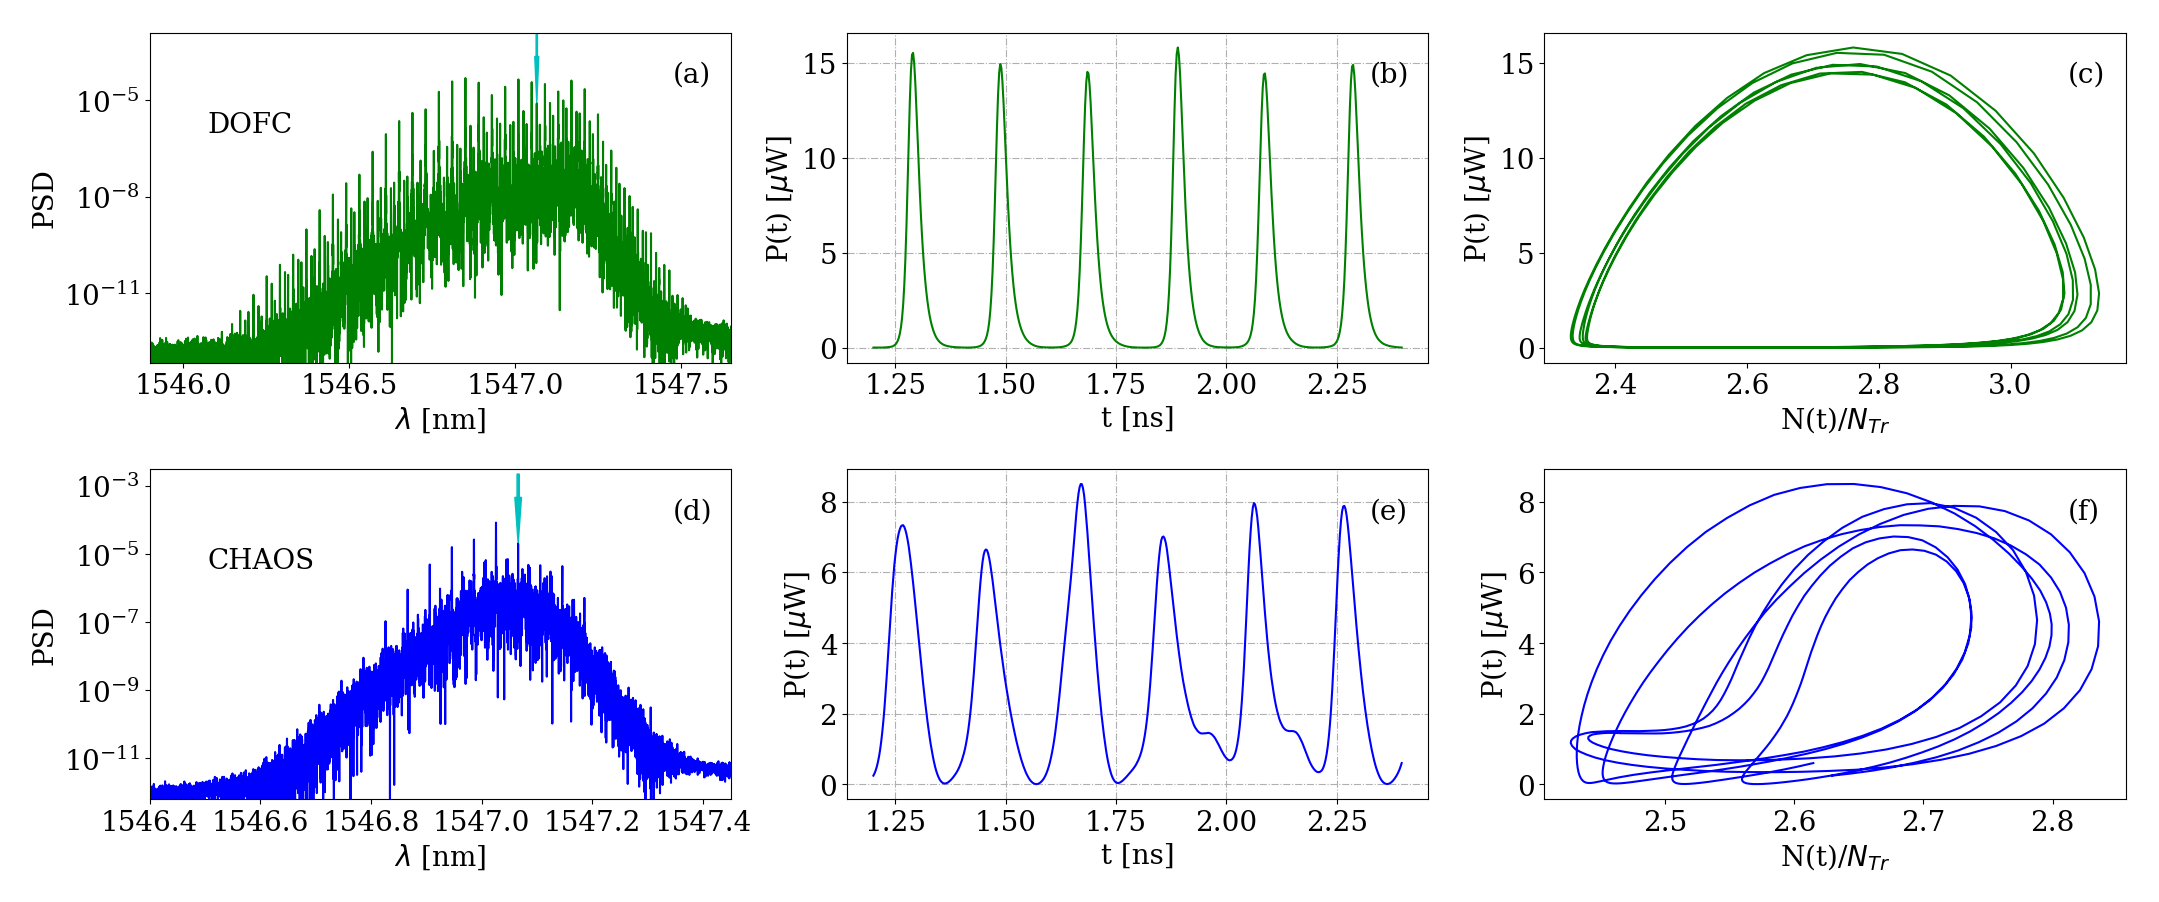
\includegraphics[width=1.0\linewidth]{chaos.png}
				\caption{\label{fig:chaos}Espectros \'opticos, $P(t)$ y atractor en el espacio de los estados de las ecuaciones de balance, despreciando los efectos de la fase \'optica; para $\delta\nu = -2$GHz y $P_{Iny} = 1\;\mu$W (DOFC, naranja) y $300\;\mu$W (CHAOS, azul).}	
			\end{figure}

		El espectro \'optico del DOFC (Figura \ref{fig:chaos} (a)) permite observar varias l\'ineas de emisión bien resultas y con una anchura entre ellas pequeña y bien definida. Ambos espectros \'opticos presentan un perfil similar formado por una ancha banda de ruido debido a la emisi\'on espont\'anea y l\'ineas de emisión que emergen de \'esta. Para el caso de CHAOS estos picos de emisi\'on son mucho menores que para el DOFC. La diferencia entre ambas regiones se hace m\'as notoria en la potencia $P(t)$, en la que para el caso del CHAOS (Figura \ref{fig:chaos} (e)) se observan oscilaciones con diferentes amplitudes para cada pido y diferentes tiempos entre \'estos. Los atractores obtenidos no dejan ninguna duda a la diferncia entre ambas regiones, obteniendo un diagrama tipo caos para $P_{Iny} = 300\;\mu$W en el que se tiende a tomar valores entodo el espacio de estados. Para el caso del DOFC se obtiene un diagrama de tipo P1 (Figura \ref{fig:chaos} (c) pero con algunas diferencias en los trazos.


			\addtocontents{toc}{\vspace{0.01cm}}
			\chapter{Conclusiones}

				Se ha realizado el desarrollo completo de un programa para la simulación de peines de frecuencia \'optica generados por l\'aseres de semiconductor. Este programa ha permitido resolver las ecuaciones de balance que modelan la interacci\'on entre los fotones y los portadores en un l\'aser de semiconductor monomodo, mediante m\'etodos de integraci\'on de ecuaciones diferenciales estoc\'asticas.

				A partir de los resultados obtenidos de la simulaci\'on se ha podido estudiar las caracter\'isticas de los OFC generados mediante las t\'ecnicas de \gs\ e inyecci\'on \'optica. El an\'alisis de los espectros \'opticos y la evoluci\'on temporal de las variables internas del l\'aser ha permitido determinar las diferentes regiones din\'amicas para distintos valores de la inyecci\'on \'optica (caracterizada por $P_{Iny}$ y $\delta\nu$). La gran precisi\'on del modelo te\'orico utilizado ha permitido obtener regiones de cambio de comportamientos correspondientes a bifurcaciones de Hopf (cambio del comportamiento IL $\rightarrow$ P1) y de doblamiento de periodo (cambio del comportamiento P1 $\rightarrow$ P2).

				El excelente acuerdo entre los resultados obtenidos de la simulaci\'on y los del experimento \cite{Chaves19} muestra la gran capacidad predictiva del mod\'elo. De esta forma, el an\'alisis computacional de la simulación permite una mejor comprensi\'on de los procesos f\'isicos involucrados en la generaci\'on de OFC. La simulaci\'on supone una importante herramienta de cara a futuros estudios m\'as detallados sobre las caracter\'isticas de los OFC generados mediante \gs\ e inyecci\'on \'optica.

				Cabe recordar que durante la simulación se ha trabajado con un tiempo transitorio, en el cu\'al se ha modificado la ecuaci\'on \ref{eq:Code-S} utilizando el t\'ermino $\sqrt{|S(t)|}$. Los buenos resultados obtenidos de la simulación avalan dicha correcci\'on. Sin embargo, puede ser interesante para futuros estudios solucionar dicho problema disminuyendo el paso de integraci\'on, sin modificar la ecuaci\'on \ref{eq:Code-S}, obteniendo soluciones m\'as rigurosas.

				Otra posible mejora del programa es el aumento de la resoluci\'on de los espectros \'opticos. \'Esto permitir\'ia estudiar la anchura de los picos de emisi\'on de los OFC, pudiendo realizar el an\'alisis de los efectos en el espectro \'optico del ruido en la fase .

		%----------------------------------------------------------------------------------------
		%     BIBLIOGRAPHY
		%----------------------------------------------------------------------------------------

			\bibliographystyle{unsrt}
			\bibliography{biblio}

		%----------------------------------------------------------------------------------------
		%     APPENDIX
		%----------------------------------------------------------------------------------------
				
			\newpage
			\appendix


				\chapter{Par\'ametros usados en la simulación}
					\label{App:params}

					En este cap\'itulo se muestran todos los par\'ametros utilizados en el programa de al simulación del trabajo. Estos par\'ametros aparecen en el script \texttt{Constants.py}, y se han obtenido de \cite{artSim} y \cite{Chaves19}.

					\begin{table}[H]
						\centering
						%\small
						\begin{tabular}{| c | c | c |}
							\hline
							S\'imbolo & Valores & Unidades \\ \hline
							$V_{act}$ & $1.53 \times 10^{-17}$ & m$^3$ \\\hline 
							$\Gamma$ & $0.06$ & - \\\hline 
							$N_{tr}$ & $1.3 \times 10^{24}$ & m$^{-3}$ \\\hline 
							$B$ & $1.5 \times 10^{16}$ & m$^3$s$^{-1}$ \\\hline 
							$\frac{\mathrm{d} g}{\mathrm{d}N}$ & $4.38 \times 10^{-20}$ & m$^2$ \\\hline 
							$\tau_p$ & $2.17$ & ps \\\hline 
							$A$ & $2.8 \times 10^8$ & s$^{-1}$ \\\hline 
							$C$ & $9.0 \times 10^{-41}$ & m$^6$s$^{-1}$ \\\hline 
							$\beta$ & $5.3 \times 10^{-6}$ & - \\\hline 
							$\eta_f$ & $0.17$ & - \\\hline 
							$\epsilon$ & $1.97 \times 10^{-23}$ & m$^3$ \\\hline 
							$\alpha$ & $3$ & - \\\hline 
							$k_c$ & $4.23 \times 10^{10}$ & s$^{-1}$ \\\hline 
							$Z_0$ & $50$ & $\Omega$ \\\hline 
							$Z_l (\textrm{a 5 GHz})$ & $92.25$ & $\Omega$ \\\hline 
							$Z_l (\textrm{a 500 MHz})$ & $53.36$ & $\Omega$ \\\hline 
							$n_g$ & $3.5$ & - \\\hline 
							$\lambda_{th}$ & $1546.843 \times 10^{-9}$ & m \\\hline 
							$I_{th}$ & $14.8$ & mA \\\hline 
						\end{tabular}
						\caption{\label{tab:param}Par\'ametros utilizados en el programa de la simulación, obtenidos a partir de \cite{artSim} y \cite{Chaves19}.}
					\end{table}

				\chapter{Código de la simulación}
					\label{App:Code}

					En este cap\'itulo se muestran partes del c\'odigo de la clase \texttt{Simulation()} desarrollada para la simulaci\'on de peines de frecuencia \'optica generados por l\'aseres de semiconductor con \gs\ e inyecci\'on de luz. No se muestra el c\'odigo completo del programa de la simulaci\'on sino solo aquellas l\'ineas de c\'odigo consideradas las m\'as importantes para entender el procedimeinto utilizado para la resoluci\'on de las ecuaciones diferenciales estoc\'asticas \ref{eq:RtEq-N}-\ref{eq:RtEq-Ph}. El resto del c\'odigo utilizado para la simulaci\'on se encuentra disponible para consulta en \cite{github}.
					
					\definecolor{gray97}{gray}{.97}
\definecolor{gray75}{gray}{.75}
\definecolor{gray45}{gray}{.45}

\lstset{ frame=Ltb,
	framerule=0pt,
	aboveskip=0.1cm,
	framextopmargin=3pt,
	framexbottommargin=3pt,
	framexleftmargin=0.4cm,
	framesep=0pt,
	rulesep=.4pt,
	backgroundcolor=\color{gray97},
	rulesepcolor=\color{black},
	%
	stringstyle=\ttfamily,
	showstringspaces = false,
	basicstyle=\small\ttfamily,
	commentstyle=\color{gray45},
	keywordstyle=\bfseries,
	%
	numbers=left,
	numbersep=15pt,
	numberstyle=\tiny,
	numberfirstline = false,
	breaklines=true,
}

\lstdefinestyle{Python}
{basicstyle=\scriptsize\bf\ttfamily,
language=python,
}

\centering\small
\vspace{0.4cm} +- - - - - - - - - - - - - 18 l\'ineas - - - - - - - - - - - - -+
\lstinputlisting[style=Python, firstline=19, lastline=26, firstnumber=19]{../src/simulation.py}
\vspace{-0.4cm} +- - - - - - - - - - - - - 18 l\'ineas - - - - - - - - - - - - -+
\lstinputlisting[style=Python, firstline=44, lastline=53, firstnumber=44]{../src/simulation.py}

\vspace{-0.4cm} +- - - - - - - - - - - - - 24 l\'ineas - - - - - - - - - - - - -+
\lstinputlisting[style=Python, firstline=77, lastline=81, firstnumber=77]{../src/simulation.py}

\vspace{-0.4cm} +- - - - - - - - - - - - - 15 l\'ineas - - - - - - - - - - - - -+
\lstinputlisting[style=Python, firstline=96, lastline=96, firstnumber=96]{../src/simulation.py}

\vspace{-0.4cm} +- - - - - - - - - - - - - 20 l\'ineas - - - - - - - - - - - - -+
\newpage
\lstinputlisting[style=Python, firstline=116, lastline=155, firstnumber=116]{../src/simulation.py}

\vspace{-0.4cm} +- - - - - - - - - - - - - 10 l\'ineas - - - - - - - - - - - - -+
\newpage
\lstinputlisting[style=Python, firstline=165, lastline=192, firstnumber=165]{../src/simulation.py}

\vspace{-0.4cm} +- - - - - - - - - - - - - 10 l\'ineas - - - - - - - - - - - - -+
\lstinputlisting[style=Python, firstline=202, lastline=206, firstnumber=202]{../src/simulation.py}

\vspace{-0.4cm} +- - - - - - - - - - - - -  6 l\'ineas - - - - - - - - - - - - -+
\lstinputlisting[style=Python, firstline=212, lastline=220, firstnumber=212]{../src/simulation.py}

\vspace{-0.4cm} +- - - - - - - - - - - - - 39 l\'ineas - - - - - - - - - - - - -+
%\lstinputlisting[style=Python, firstline=96, lastline=220, firstnumber=100]{../src/simulation.py}

	\end{document}

%----------------------------------------------------------------------------------------
%              END
%----------------------------------------------------------------------------------------
